\documentclass[lettersize,journal]{IEEEtran}
\usepackage{amsmath,amsfonts}
\usepackage{algorithmic}
\usepackage{algorithm}
\usepackage{array}
\usepackage[caption=false,font=normalsize,labelfont=sf,textfont=sf]{subfig}
\usepackage{textcomp}
\usepackage{stfloats}
\usepackage{url}
\usepackage{verbatim}
\usepackage{graphicx}
\usepackage{cite}

\usepackage{multirow}
\usepackage{booktabs}
%\usepackage{subcaption}
\usepackage{caption}
\usepackage[dvipsnames]{xcolor} % 更全的色系
\usepackage{listings} % 排代码用的宏包
\usepackage[framed,numbered,autolinebreaks,useliterate]{mcode}

\hyphenation{op-tical net-works semi-conduc-tor IEEE-Xplore}
% updated with editorial comments 8/9/2021

\makeatletter
\newcommand{\rmnum}[1]{\romannumeral #1}
\newcommand{\Rmnum}[1]{\expandafter\@slowromancap\romannumeral #1@}
\makeatother


\begin{document}

\title{Lab 2: Power System Optimization}

\author{Ran Zhang, College of Electrical Engineering, Zhejiang University \\Student ID: 22310173
}


% The paper headers
\markboth{Journal of \LaTeX\ Class Files,~Vol.~14, No.~8, August~2021}%
{Shell \MakeLowercase{\textit{et al.}}: A Sample Article Using IEEEtran.cls for IEEE Journals}

\maketitle

\begin{abstract}
This report delves into power system optimization through single-period optimal power flow (OPF), multi-period OPF, and security-constrained unit commitment (SCUC), utilizing YALMIP, MATLAB, and Cplex for computational implementation. These optimization techniques aim to enhance the operation of power systems while considering various constraints and objectives. Through experimentation and analysis using YALMIP, MATLAB, and Cplex, valuable insights are gained into power system operation and management, with implications for improving efficiency, reliability, and sustainability. The results contribute to advancing power system optimization methodologies, informing decision-making in power grid operation and planning.
\end{abstract}

\begin{IEEEkeywords}
Power system optimization, security-constrained unit commitment (SCUC), optimal power flow (OPF).
\end{IEEEkeywords}

\section{Introduction}
\IEEEPARstart{T}{he} efficient and reliable operation of power systems is paramount for ensuring the uninterrupted supply of electricity to meet the demands of modern society. Power system optimization plays a crucial role in achieving this objective by effectively managing the generation, transmission, and distribution of electrical energy while considering various constraints and objectives.

Single-period OPF focuses on optimizing the generation and dispatch of power resources within a single time period to minimize total generation cost while ensuring the satisfaction of power flow constraints and system limitations. Multi-period OPF extends this analysis to optimize generation schedules over multiple time periods, accounting for time-varying demand patterns and generation constraints.

The SCUC problem adds an additional layer of complexity by incorporating security constraints to guarantee the reliability and stability of the power system under various operating conditions and contingencies. It involves determining the optimal commitment and dispatch of generation units while considering factors such as transmission constraints, reserve requirements, and potential contingencies.

Through a comprehensive exploration of single-period OPF, multi-period OPF, and SCUC, this report aims to provide insights into the optimization of power system operation, contributing to the advancement of sustainable and resilient energy systems.

In power system optimization, YALMIP is often used for formulating optimization models due to its ease of use and flexibility. Users can define the objective function, constraints, and decision variables using MATLAB syntax, leveraging YALMIP's optimization modeling capabilities. Once the optimization model is formulated, Cplex is employed as the solver to efficiently solve the optimization problem and obtain optimal solutions. Cplex's advanced algorithms and computational efficiency enable it to handle large-scale power system optimization problems with ease, providing accurate and reliable solutions in a timely manner.

Overall, the combination of YALMIP and Cplex provides a powerful platform for formulating and solving complex optimization problems encountered in power system optimization, enabling researchers and practitioners to address operational challenges and improve the performance and reliability of power grids.



\section{Single-period OPF}
Single-period OPF only considers one time interval and dispatches all the online generators to supply the demand while minimizing the total operating cost. In this task, there will be three step to finish this problem.

\subsection{Use YALMIP to establish the single-period OPF model above and optimize using Cplex solver}
A modified version of the IEEE 39-bus system, referred to as "case39ee m," is provided as an attachment. This file contains data related to generator specifications, bus configurations, and branch parameters. Additionally, for a comprehensive understanding of the variables utilized within the system, the file "scaseformat.m" in the MATPOWER package provides definitions and units for these variables.
\subsubsection{Data processing}
Firstly, import the system parameters and data from \textit{case39ee.m} as \textit{mpc}, which is called textit{Data Processing}. Then obtain $B^{bus}, B^f$ using \textit{makeBdc} function in MATPOWER. After that, form the generator matrix based on the instruction.

\begin{lstlisting}[]
	mpc = case39ee;
	bus=mpc.bus;
	gen=mpc.gen;
	branch=mpc.branch;
	gencost=mpc.gencost;
	baseMVA=mpc.baseMVA;
	
	% Form Bbus, Bf
	[Bbus, Bf, Pbusinj, Pfinj] = makeBdc(baseMVA, bus, branch);
	
	% Form Cg (Generator matrix)
	col=gen(:,1);
	Cg=zeros(Nbus,Nunits);
	for i=1:Nunits
		Cg(col(i),i)=1;
	end
\end{lstlisting}

In addition, $B^{bus}, B^f$ can also be obtained by the following formula:
\begin{align}
	&B^f = B^{ff}(C^f-C^t)\\
	&B^{bus} = (C^f-C^t)^TB^f
\end{align}

$B^{ff}$ is a sparse matrix. Utilizing the sparse matrix can significantly reduce the required storage space, making it particularly advantageous for analyzing large systems.

Then, use the mathematical model from the instruction file, the optimization problem is described as follows.

\subsubsection{Objective}

For the purpose of simplicity, we use linear cost function for each generator:
\begin{equation}
	f=\sum_{i=1}^{NG}(c_i^ox_i+c_i^l)
\end{equation}
Type this equation in MATLAB using YALMIP. $Horizon$ is 1 for Single-period (Horizon is reserved here for the convenience of expansion). $x$ is is the power output from generator. $theta$ is the voltage angle of bus.
\begin{lstlisting}[]
%% OPF Model
	x = sdpvar(Nunits,Horizon,'full');
	theta=sdpvar(Nbus,Horizon,'full');
	Objective = 0;
	for k = 1:Horizon
		Objective = Objective + C*x(:,k);
	end
	Objective = Objective +sum(Cl);
\end{lstlisting}

\subsubsection{Constraints}

After that, use for-loops to add constraints one by one. $C^g$ is the generator connection matrix, \textit{Pforecast} comes from \textit{mpc} and divided by \textit{baseMVA} and $F^{max}$ comes from long term rating of branches.
\begin{lstlisting}[]
	Constraints = [];
	for k = 1:Horizon
	Constraints = [Constraints, Pmin <= x(:,k) <= Pmax];
	end
	balanceL=Bbus*theta;
	balanceR=Cg*x-Pforecast*LoadRatio;
	Constraints = [Constraints, balanceL == balanceR];
	Constraints = [Constraints, -PLmax*LoadRatio<=Bf*theta...
		<=PLmax*LoadRatio];
	slack = find(bus(:,2)==3);
	Constraints = [Constraints, theta(slack)==0];
	
\end{lstlisting}
\subsubsection{Optimization}
Lastly,  optimize and analyze the model.
\begin{lstlisting}
	ops = sdpsettings('solver', 'cplex');
	optimize(Constraints, Objective, ops)
	rl=Bf*value(theta)./(PLmax*LoadRatio)
	ObMy=value(Objective) % Used to show the value of optimization problem
\end{lstlisting}

The generation result is shown in the Fig. 1. Other results are shown in Fig. 2. From Fig.2, it can be seen that the optimization problem is solved successfully, and the optimal cost(Objective in this problem) is 35069.31 \$/MWh
\begin{figure}[htbp]
	\centering
	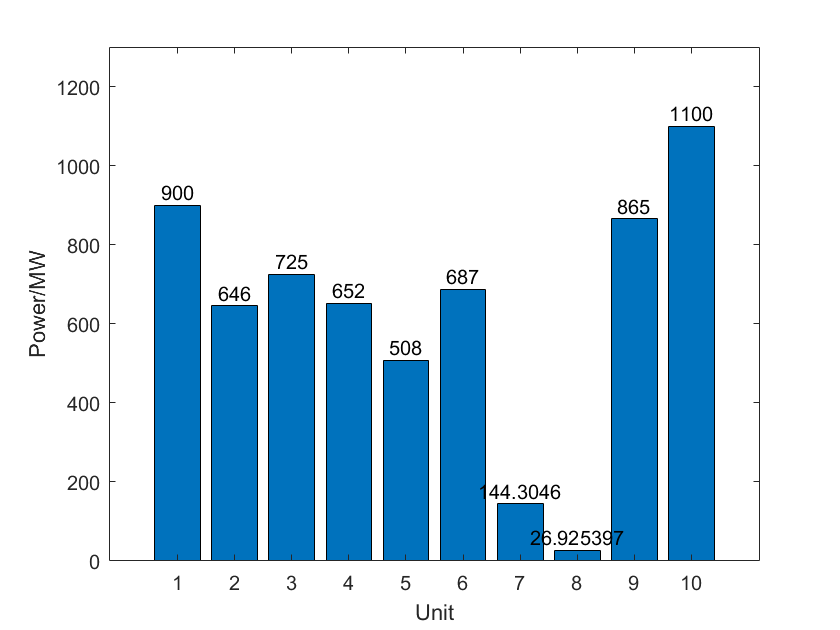
\includegraphics[width=0.5\textwidth]{t1-gen}
	\caption{Output of single-period OPF
	}
	\label{fig_1}
\end{figure}

\begin{figure}[htbp]
	\centering
	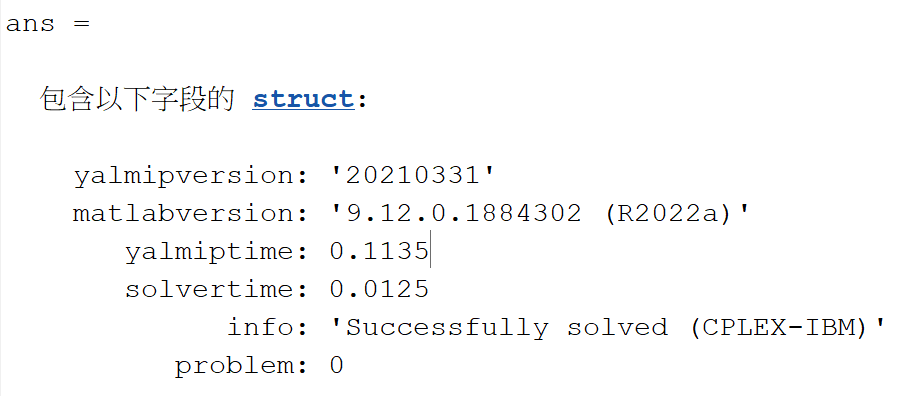
\includegraphics[width=0.5\textwidth]{t1-ans}
	\caption{Solver information for single-period OPF
	}
	\label{fig_2}
\end{figure}

\subsection{Use “rundcopf” function in MATPOWER to solve the same problem again so as to verify the results from Step a)}
The code using “rundcopf” function in MATPOWER is shown as follows.
\begin{lstlisting}
	mpopt=mpoption;
	mpopt = mpoption(mpopt);
	rundcopf(mpc)
\end{lstlisting}


The provided code snippet initializes MATPOWER options and then executes a DC optimal power flow (DCOPF) analysis on the specified power system. The DCOPF problem optimizes active power generation and bus voltage angles under linearized power flow equations. The input data structure contains information about the power system, including generator and load data, branch parameters, and network topology.

% Table generated by Excel2LaTeX from sheet 'MAT VS MY'
\begin{table*}[htbp]
	\centering
	\caption{Comparison of branch flow between results from Step A and MATPOWER}
	\begin{tabular}{cccccc}
		\toprule
		Branch & From Bus & To Bus & Step A(MW) + Cplex & Step A(MW) + GLPK & \multicolumn{1}{c}{MATPOWER(MW)} \\
		\midrule
		1     & 1     & 2     & -141.1545476 & -141.1545476 & -141.1545476 \\
		\midrule
		2     & 1     & 39    & 43.5545476 & 43.5545476 & 43.5545476 \\
		\midrule
		3     & 2     & 3     & 500   & 500   & 500 \\
		\midrule
		4     & 2     & 25    & 258.8454524 & 258.8454524 & 258.8454524 \\
		\midrule
		5     & 2     & 30    & -900  & -900  & -900 \\
		\midrule
		6     & 3     & 4     & 54.73318697 & 54.73318697 & 54.73318697 \\
		\midrule
		7     & 3     & 18    & 123.266813 & 123.266813 & 123.266813 \\
		\midrule
		8     & 4     & 5     & -234.4055142 & -234.4055142 & -234.4055142 \\
		\midrule
		9     & 4     & 14    & -210.8612989 & -210.8612989 & -210.8612989 \\
		\midrule
		10    & 5     & 6     & -534.7298948 & -534.7298948 & -534.7298948 \\
		\midrule
		11    & 5     & 8     & 300.3243807 & 300.3243807 & 300.3243807 \\
		\midrule
		12    & 6     & 7     & 422.4210717 & 422.4210717 & 422.4210717 \\
		\midrule
		13    & 6     & 11    & -320.3509666 & -320.3509666 & -320.3509666 \\
		\midrule
		14    & 6     & 31    & -636.8 & -636.8 & -636.8 \\
		\midrule
		15    & 7     & 8     & 188.6210717 & 188.6210717 & 188.6210717 \\
		\midrule
		16    & 8     & 9     & -33.0545476 & -33.0545476 & -33.0545476 \\
		\midrule
		17    & 9     & 39    & -39.5545476 & -39.5545476 & -39.5545476 \\
		\midrule
		18    & 10    & 11    & 328.0054371 & 328.0054371 & 328.0054371 \\
		\midrule
		19    & 10    & 13    & 396.9945629 & 396.9945629 & 396.9945629 \\
		\midrule
		20    & 10    & 32    & -725  & -725  & -725 \\
		\midrule
		21    & 12    & 11    & -7.654470543 & -7.654470543 & -7.654470543 \\
		\midrule
		22    & 12    & 13    & -0.875529457 & -0.875529457 & -0.875529457 \\
		\midrule
		23    & 13    & 14    & 396.1190334 & 396.1190334 & 396.1190334 \\
		\midrule
		24    & 14    & 15    & 185.2577346 & 185.2577346 & 185.2577346 \\
		\midrule
		25    & 15    & 16    & -134.7422654 & -134.7422654 & -134.7422654 \\
		\midrule
		26    & 16    & 17    & 17.46233798 & 17.46233798 & 17.46233798 \\
		\midrule
		27    & 16    & 19    & -480  & -480  & -480 \\
		\midrule
		28    & 16    & 21    & -140.7572856 & -140.7572856 & -140.7572856 \\
		\midrule
		29    & 16    & 24    & 139.5526822 & 139.5526822 & 139.5526822 \\
		\midrule
		30    & 17    & 18    & 34.73318697 & 34.73318697 & 34.73318697 \\
		\midrule
		31    & 17    & 27    & -17.27084898 & -17.27084898 & -17.27084898 \\
		\midrule
		32    & 19    & 20    & 172   & 172   & 172 \\
		\midrule
		33    & 19    & 33    & -652  & -652  & -652 \\
		\midrule
		34    & 20    & 34    & -508  & -508  & -508 \\
		\midrule
		35    & 21    & 22    & -414.7572856 & -414.7572856 & -414.7572856 \\
		\midrule
		36    & 22    & 23    & 272.2427144 & 272.2427144 & 272.2427144 \\
		\midrule
		37    & 22    & 35    & -687  & -687  & -687 \\
		\midrule
		38    & 23    & 24    & 169.0473178 & 169.0473178 & 169.0473178 \\
		\midrule
		39    & 23    & 36    & -144.3046034 & -144.3046034 & -144.3046034 \\
		\midrule
		40    & 25    & 26    & 61.77084898 & 61.77084898 & 61.77084898 \\
		\midrule
		41    & 25    & 37    & -26.92539658 & -26.92539658 & -26.92539658 \\
		\midrule
		42    & 26    & 27    & 298.270849 & 298.270849 & 298.270849 \\
		\midrule
		43    & 26    & 28    & -162.8652 & -162.8652 & -162.8652 \\
		\midrule
		44    & 26    & 29    & -212.6348 & -212.6348 & -212.6348 \\
		\midrule
		45    & 28    & 29    & -368.8652 & -368.8652 & -368.8652 \\
		\midrule
		46    & 29    & 38    & -865  & -865  & -865 \\
		\bottomrule
	\end{tabular}%
	\label{tab:addlabel}%
\end{table*}%


% Table generated by Excel2LaTeX from sheet 'MAT VS MY'
\begin{table*}[htbp]
	\centering
	\caption{Comparison of generators' output between results from Step A and MATPOWER}
	\begin{tabular}{ccccc}
		\toprule
		Bus   & Generator & Step A(MW) + Cplex & Step A(MW) + GLPK & MATPOWER(MW) \\
		\midrule
		30    & 1     & 900   & 900   & 900 \\
		\midrule
		31    & 2     & 646   & 646   & 646 \\
		\midrule
		32    & 3     & 725   & 725   & 725 \\
		\midrule
		33    & 4     & 652   & 652   & 652 \\
		\midrule
		34    & 5     & 508   & 508   & 508 \\
		\midrule
		35    & 6     & 687   & 687   & 687 \\
		\midrule
		36    & 7     & 144.3046 & 144   & 144.3046 \\
		\midrule
		37    & 8     & 26.9254 & 27    & 26.9254 \\
		\midrule
		38    & 9     & 865   & 865   & 865 \\
		\midrule
		39    & 10    & 1100  & 1100  & 1100 \\
		\bottomrule
	\end{tabular}%
	\label{tab:addlabel}%
\end{table*}%


In the DC power flow model, the voltage magnitude is assumed to be constant at 1.0, and the reactive power is assumed to be 0. Therefore, these two parameters are not explicitly listed in the model. TABLE \Rmnum{1} and TABLE \Rmnum{2} compare the results from Step A and MATPOWER.

From TABLE I and TABLE II, it is apparent that the results obtained using GLPK and MATPOWER are nearly identical, except for a slight variation in generator output. However, the results obtained using CPLEX are precisely the same as those from MATPOWER. Therefore, any discrepancies observed between GLPK and MATPOWER results can be attributed to solver inaccuracies.

\subsection{Change load ratio and observe the change in branch loading rate and generator power output}

In this step, the load ratio is varied between 0.8, 1, and 1.1, and the corresponding changes in branch loading rate and generator power output are observed. The objective is to analyze the influence of the load ratio on optimal power flow (OPF) solutions.

Branch loading rate can be calculated as follows:
\begin{equation}
	r_l=\frac{F_l}{F_l^{\max}}=\frac{\sum_j^{NB}B_{lj}^f\theta_j}{F_l^{\max}}\quad\forall l\in\{1,\cdots,NL\}
\end{equation}


Therefore, in MATLAB the code should be changed as follows:
\begin{lstlisting}
	% Set load ratio (Task C)
	LoadRatio=1;
	Constraints = [Constraints, -PLmax*LoadRatio<=Bf*theta...
		<=PLmax*LoadRatio];
	rl=Bf*value(theta)./(PLmax*LoadRatio)
\end{lstlisting}

So that we could get Generator power output at different load ratio, as shown in TABLE \Rmnum{3}. The data of change in branch loading rate is shown in Fig. 2.

% Table generated by Excel2LaTeX from sheet 'Sheet2'
\begin{table}[htbp]
	\centering
	\caption{Generator power output at different load ratio}
	\begin{tabular}{ccccc}
		\toprule
		&       & \multicolumn{3}{c}{Load ratio} \\
		\midrule
		Bus   & Generator & 0.8   & 1     & 1.1 \\
		\midrule
		30    & 1     & 707.563 & 900   & 990 \\
		\midrule
		31    & 2     & 622.0794 & 646   & 646 \\
		\midrule
		32    & 3     & 720   & 725   & 725 \\
		\midrule
		33    & 4     & 652   & 652   & 652 \\
		\midrule
		34    & 5     & 0     & 508   & 508 \\
		\midrule
		35    & 6     & 687   & 687   & 687 \\
		\midrule
		36    & 7     & 0     & 144.3046 & 570.9862 \\
		\midrule
		37    & 8     & 0     & 26.9254 & 135.6668 \\
		\midrule
		38    & 9     & 514.7416 & 865   & 865 \\
		\midrule
		39    & 10    & 1100  & 1100  & 1100 \\
		\bottomrule
	\end{tabular}%
	\label{tab:addlabel}%
\end{table}%


\begin{figure}[htbp]
	\centering
	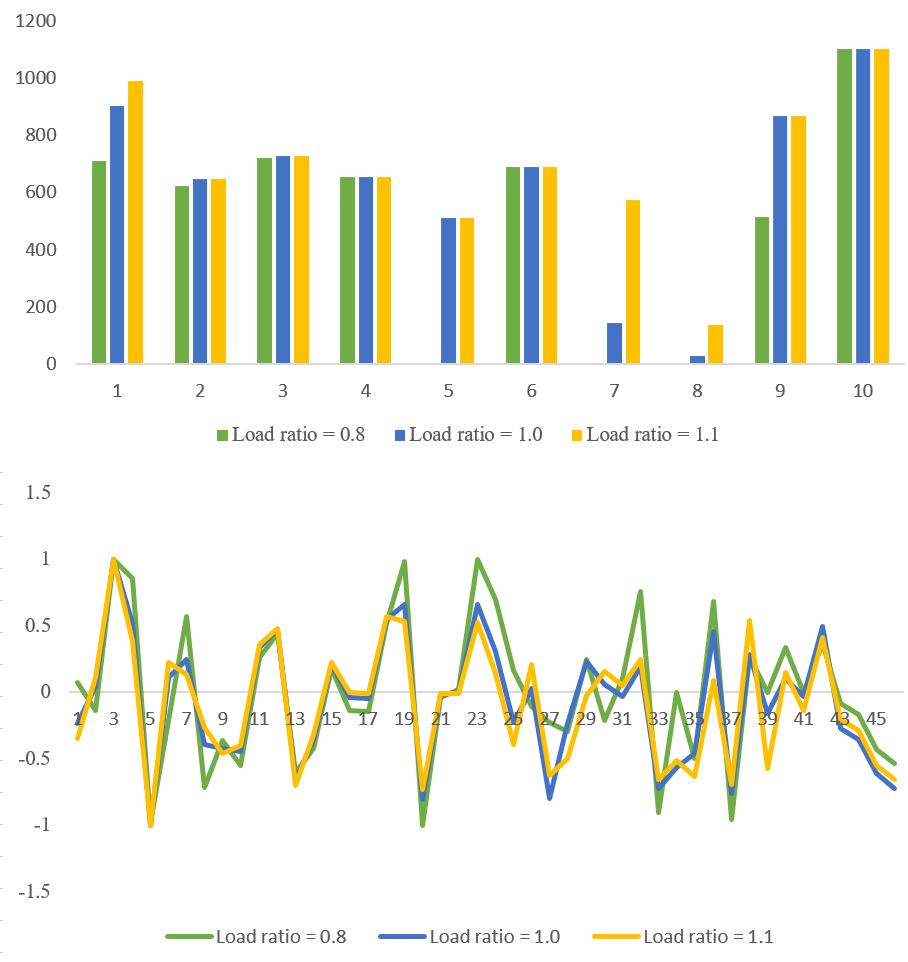
\includegraphics[width=0.5\textwidth]{t1-loadratio}
	\caption{The impact of load ratio on generator output and branch loading rate}
	\label{fig_2}
\end{figure}


From Figure 2 and TABLE 2, it is evident that as the load ratio increases, more generators become active within the system. When the load ratio is too low, there is a risk of some generators being forced to shut down due to insufficient demand (like Generator 5, 7 and 8 when load ratio is 0.8). Conversely, when the load ratio is too high, nearly all generators are required to operate at maximum power output to meet the increased demand.

The impact of load ratio on branch loading rate reveals distinct trends are as follows:

$\bullet$ With an increase in load ratio, certain branches (4, 5, 7, 8, 16, 17, 19, 23, 24, 40) experience a decrease in absolute loading rates, indicating reduced power flow.

$\bullet$ Conversely, an increase in load ratio leads to increased loading rates for more branches (1, 6, 9, 10, 11, 12, 13, 14, 15, 18, 25, 27, 28, 35, 37, 41), indicating heightened power flow.

$\bullet$ Notably, for some branches (2, 6, 26, 30), the direction of loading rate is altered with changing load ratios.

$\bullet$ The total absolute flow on the branches under the three load ratios are 11341 MW, 12963 MW, and 14199 MW, respectively.

Overall, while the increase in load ratio may not uniformly influence the power flow direction of each branch due to varying sensitivities, the total power flow across all branches tends to increase.

\section{Multi-period OPF}
In this task, we upgrade the single-period OPF model into multi-period, while consider wind power generation as well as generator ramping constraints.
\subsection{Use YALMIP to establish the multi-period OPF model and optimize}
\subsubsection{Data processing}
A modified IEEE 39-bus system is selected as test system, wind generator is installed on bus 14. Load data and wind perdition data is stored in the "Data for multi-period OPF" sheet of the DATA.xlsx. Set the load ratio to 1. So the first step is processing the data from excel, which is shown as follows:
\begin{lstlisting}
	opts = spreadsheetImportOptions...
		("NumVariables", 2);
	opts.Sheet = "Datas for multi-period OPF";
	opts.DataRange = "C2:D25";
	opts.VariableNames = ["Load", "wind"];
	opts.VariableTypes = ["double", "double"];
	Wind = readtable("DATA.xlsx", opts, "UseExcel", false);
	Wind=table2array(Wind);
	clear opts
\end{lstlisting}

Then set load rate and wind rate.
\begin{lstlisting}
	LoadRate=Wind(:,1)';
	Pforecast=bus(:,3)*LoadRate; % T=24 Load
	
	WindRate=0.1;
	TotalGen=WindRate*sum(Pmax);
	Pw=Wind(:,2)*TotalGen;  % The predicted output of wind generator
	Pw=Pw';
\end{lstlisting}

\subsubsection{Objective}
Firstly, add decision variables. $xw$ represents the actual output of the wind generator, which should be included indecision variables.
\begin{lstlisting}
	x = sdpvar(Nunits,Horizon,'full');
	theta=sdpvar(Nbus,Horizon,'full');
	xw= sdpvar(1,Horizon,'full');
\end{lstlisting}

Then rewrite the objective function. In this new function, multi-period cost function and the cost of wind curtailment are considered.

\begin{lstlisting}
	Objective = 0;
	% Obj  f1
	for k = 1:Horizon
	Objective = Objective + C*x(:,k);
	end
	Objective = Objective +sum(Cl) * Horizon;
	% Obj f2
	Lambda=10;
	f2=sum(Pw-xw);
	f2=f2*Lambda;
	Objective=Objective+f2;
\end{lstlisting}

\subsubsection{Constraints}
 The output of wind generator is added into nodal power balance constraints as Line 1-5, with additional term added into the nodal power balance constraints. Generator ramping constraints and wind curtailment constraints are also added in this optimization problem. Other constraints stay the same.
\begin{lstlisting}
	% Generator constraints
	Constraints = [];
	for k = 1:Horizon
	Constraints = [Constraints, Pmin <= x(:,k) <= Pmax];
	end
	
	%Balancing constraints
	balanceL=Bbus*theta;
	balanceR=Cg*x + Cw*xw-Pforecast*LoadRatio;
	Constraints = [Constraints, balanceL == balanceR];
	for k = 1:Horizon
	temp = Bf*theta;
	Constraints = [Constraints, -PLmax*LoadRatio<=temp(:,k)<=...
		PLmax*LoadRatio];
	end
	
	% slack bus
	slack = find(bus(:,2)==3);
	Constraints = [Constraints, theta(slack)==0];
	
	% Ramping constraints
	Eta=0.7;
	RD=Eta*Pmax;
	RU=RD;
	for k = 2: Horizon
	Constraints = [Constraints, -RD<= (x(:,k)-  x(:,k-1)) <= RU ];
	end
	
	% Wind generator constraints
	Constraints = [Constraints, 0<= xw <= Pw ];
\end{lstlisting}

\subsubsection{Optimization}
Lastly,  optimize and analyze the model.
\begin{lstlisting}
	ops = sdpsettings('solver', 'cplex');
	optimize(Constraints, Objective, ops) % Set the solver to cplex
\end{lstlisting}
Fig. 4 illustrates the power output of both common and wind generators, alongside the forecasted load when wind rate is 0.1.

Observing the power output of generators alongside the branch loading rate across different time intervals reveals significant insights into the system dynamics.  Notably, the aggregate output of generators demonstrates a capability to closely track the system load over time. It's noteworthy that in this scenario, there is no curtailment of wind power. Additionally, generators 1, 3, 4, and 9 exhibit minimal variation in output concerning load fluctuations, indicating their role in supplying the base load. Conversely, the output of other generators shows a proportional increase with the rising load. At lower loads, certain generators may cease operation, resulting in zero output.

Turning attention to the branch loading rate, Fig.5 provides insights into the loading status of individual transmission lines. Broadly categorized, the branch loading rate exhibits four distinct patterns. Firstly, there are branches, such as 5 and 22, where the loading rate remains relatively constant regardless of load variations. Secondly, branches like 10 and 12 display a synchronous variation pattern with the load, indicating a direct correlation between load changes and branch loading. In contrast, the third type, represented by branches 4 and 32, exhibits an inverse relationship with the load, where the loading rate fluctuates in the opposite direction to the load changes. Finally, the fourth type demonstrates a more complex behavior, where the branch loading rate varies with the load, albeit without discernible regularity.

By understanding these patterns, system operators can gain valuable insights into the dynamic interplay between generator output, load demand, and transmission line loading, enabling more effective grid management and operational decision-making.

\begin{figure}
	\centering
	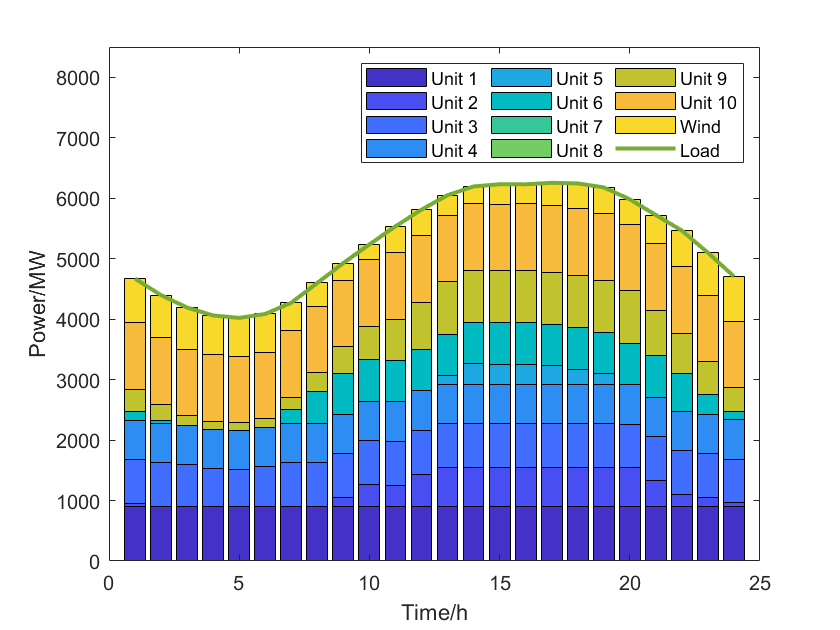
\includegraphics[width=0.5\textwidth]{t2-windrate0.1}
	\caption{The generator output for different time intervals (wind rate = 0.1)}
	\label{fig_4}
\end{figure}

\begin{figure}
	\centering
	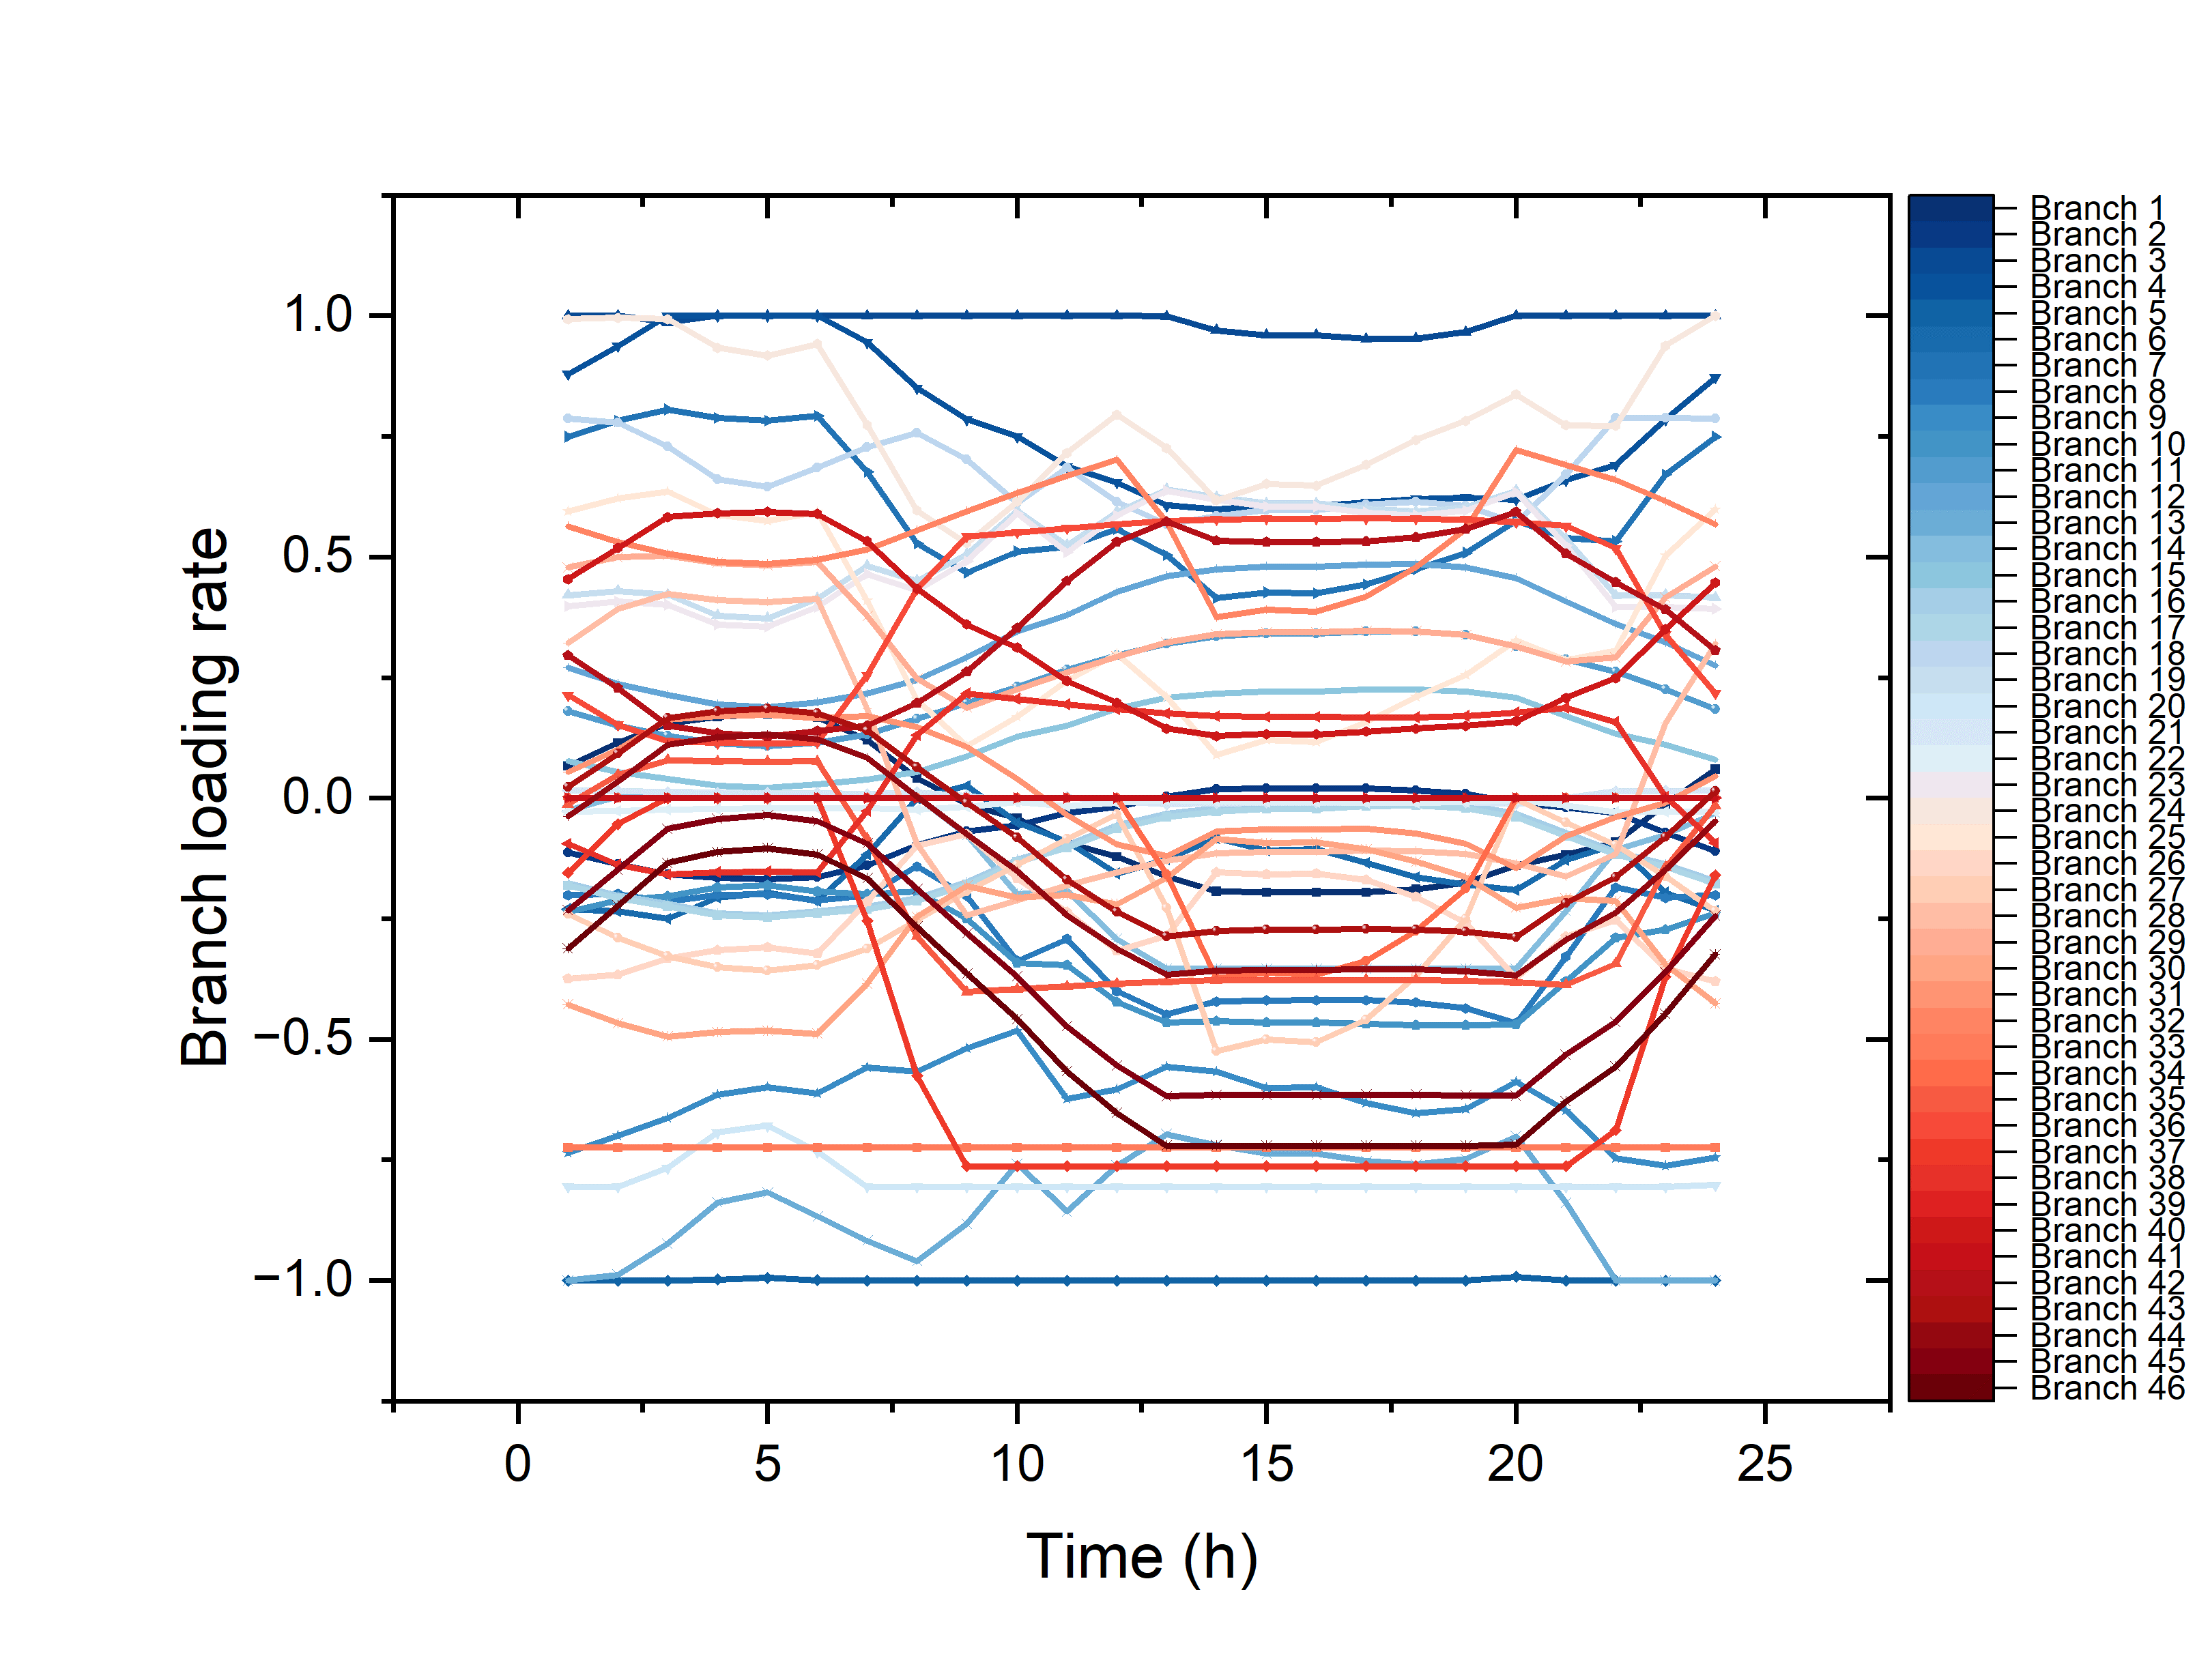
\includegraphics[width=0.5\textwidth]{t2-br-wr0.1}
	\caption{The branch loading rate for different time intervals (wind rate = 0.1)}
	\label{fig_2}
\end{figure}

\begin{figure}
	\centering
	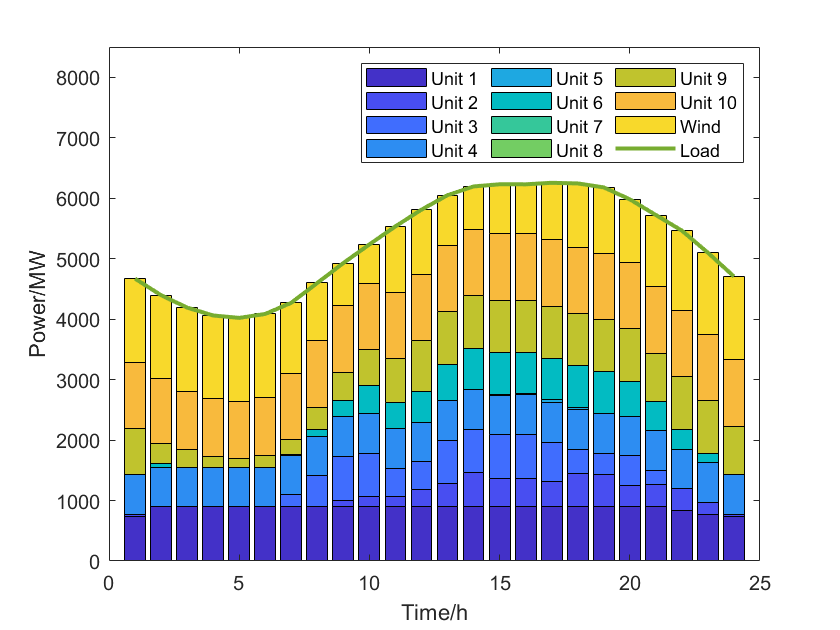
\includegraphics[width=0.5\textwidth]{t2-windrate0.25}
	\caption{The generator output for different time intervals (wind rate = 0.25)}
	\label{fig_4}
\end{figure}
\subsection{Increase the capacity of the wind generator to 25\% and 50\%}

\begin{figure}
	\centering
	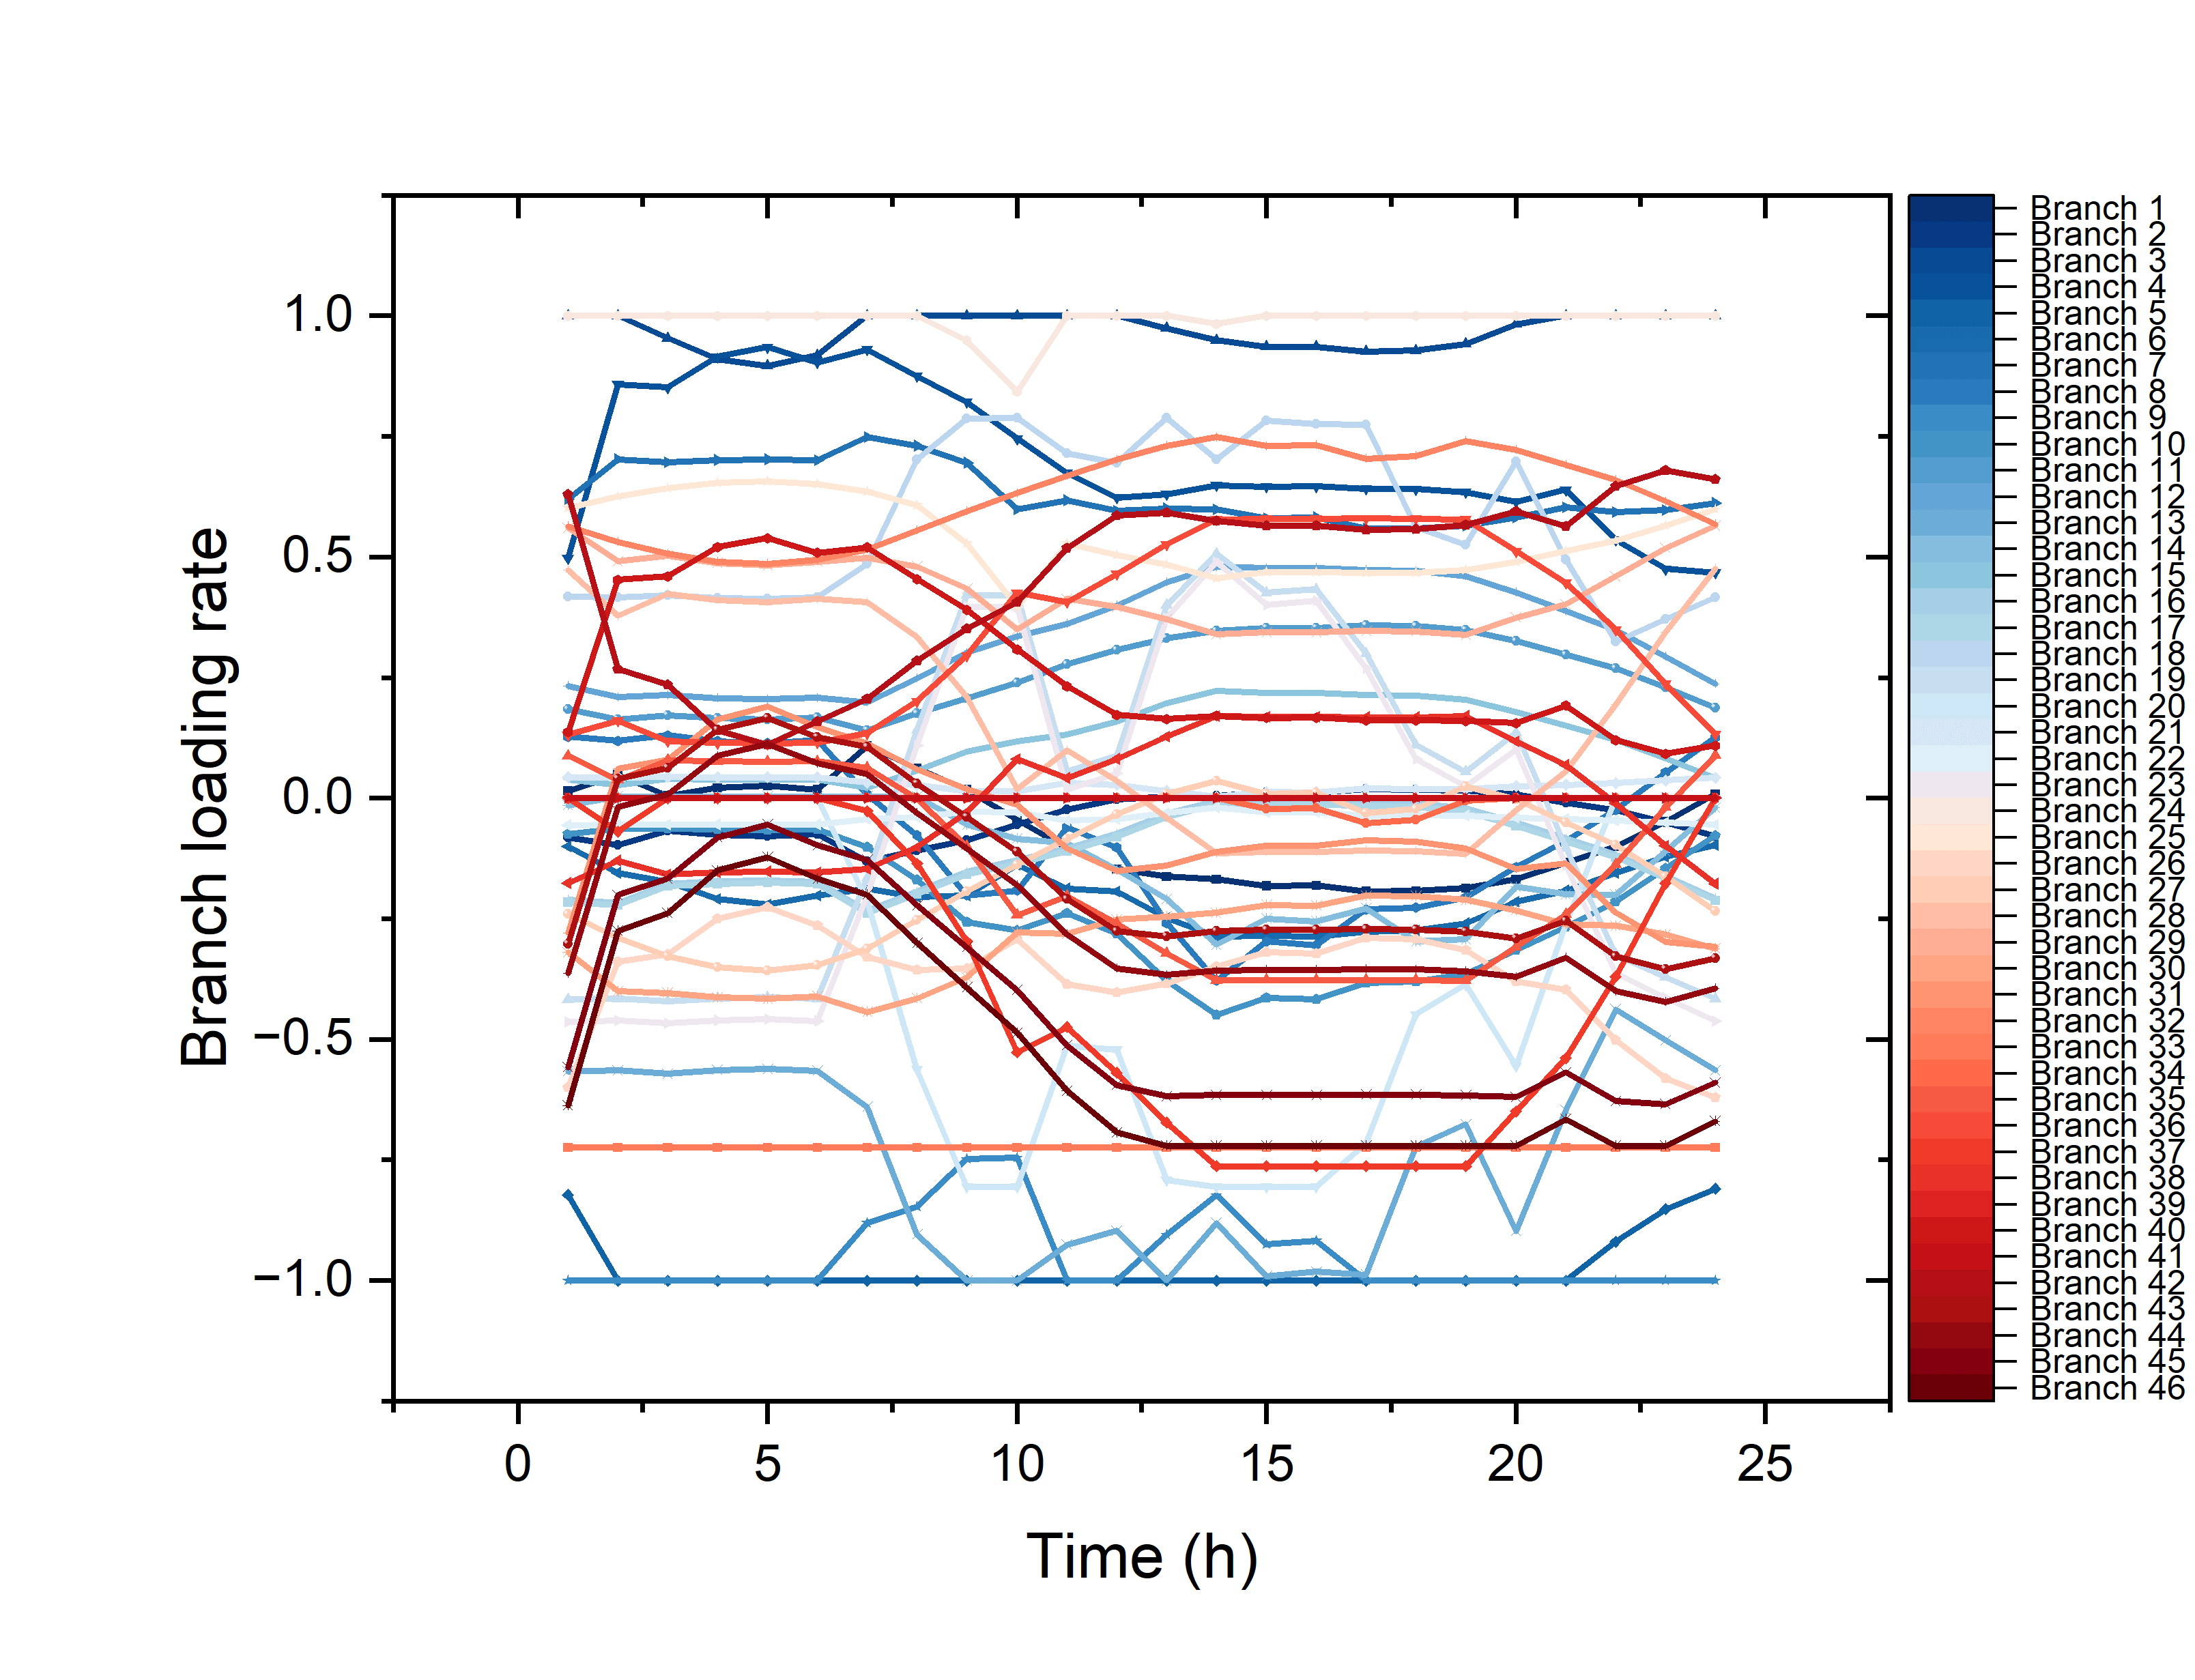
\includegraphics[width=0.5\textwidth]{t2-br-wr0.25}
	\caption{The branch loading rate for different time intervals (wind rate = 0.25)}
	\label{fig_2}
\end{figure}

\begin{figure}
	\centering
	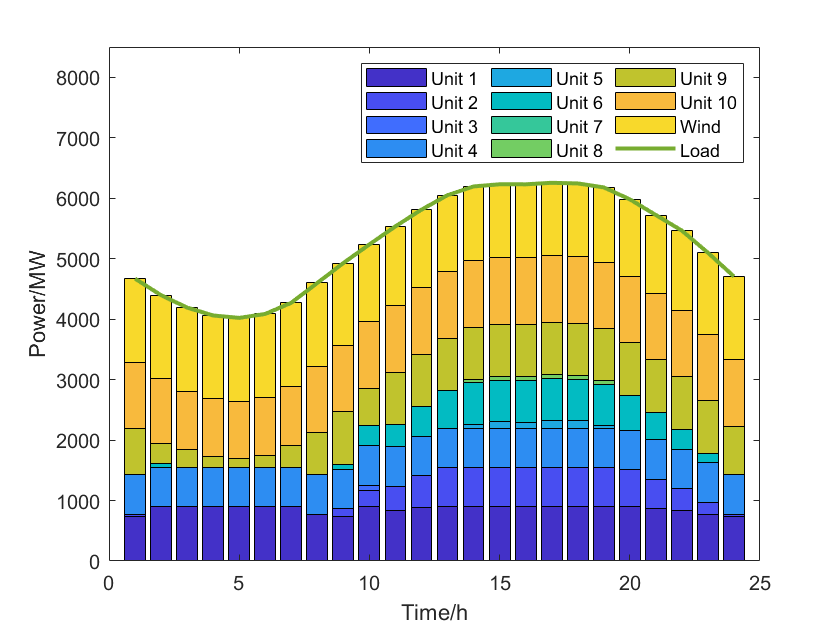
\includegraphics[width=0.5\textwidth]{t2-windrate0.5}
	\caption{The generator output for different time intervals (wind rate = 0.5)}
	\label{fig_4}
\end{figure}

\begin{figure}
	\centering
	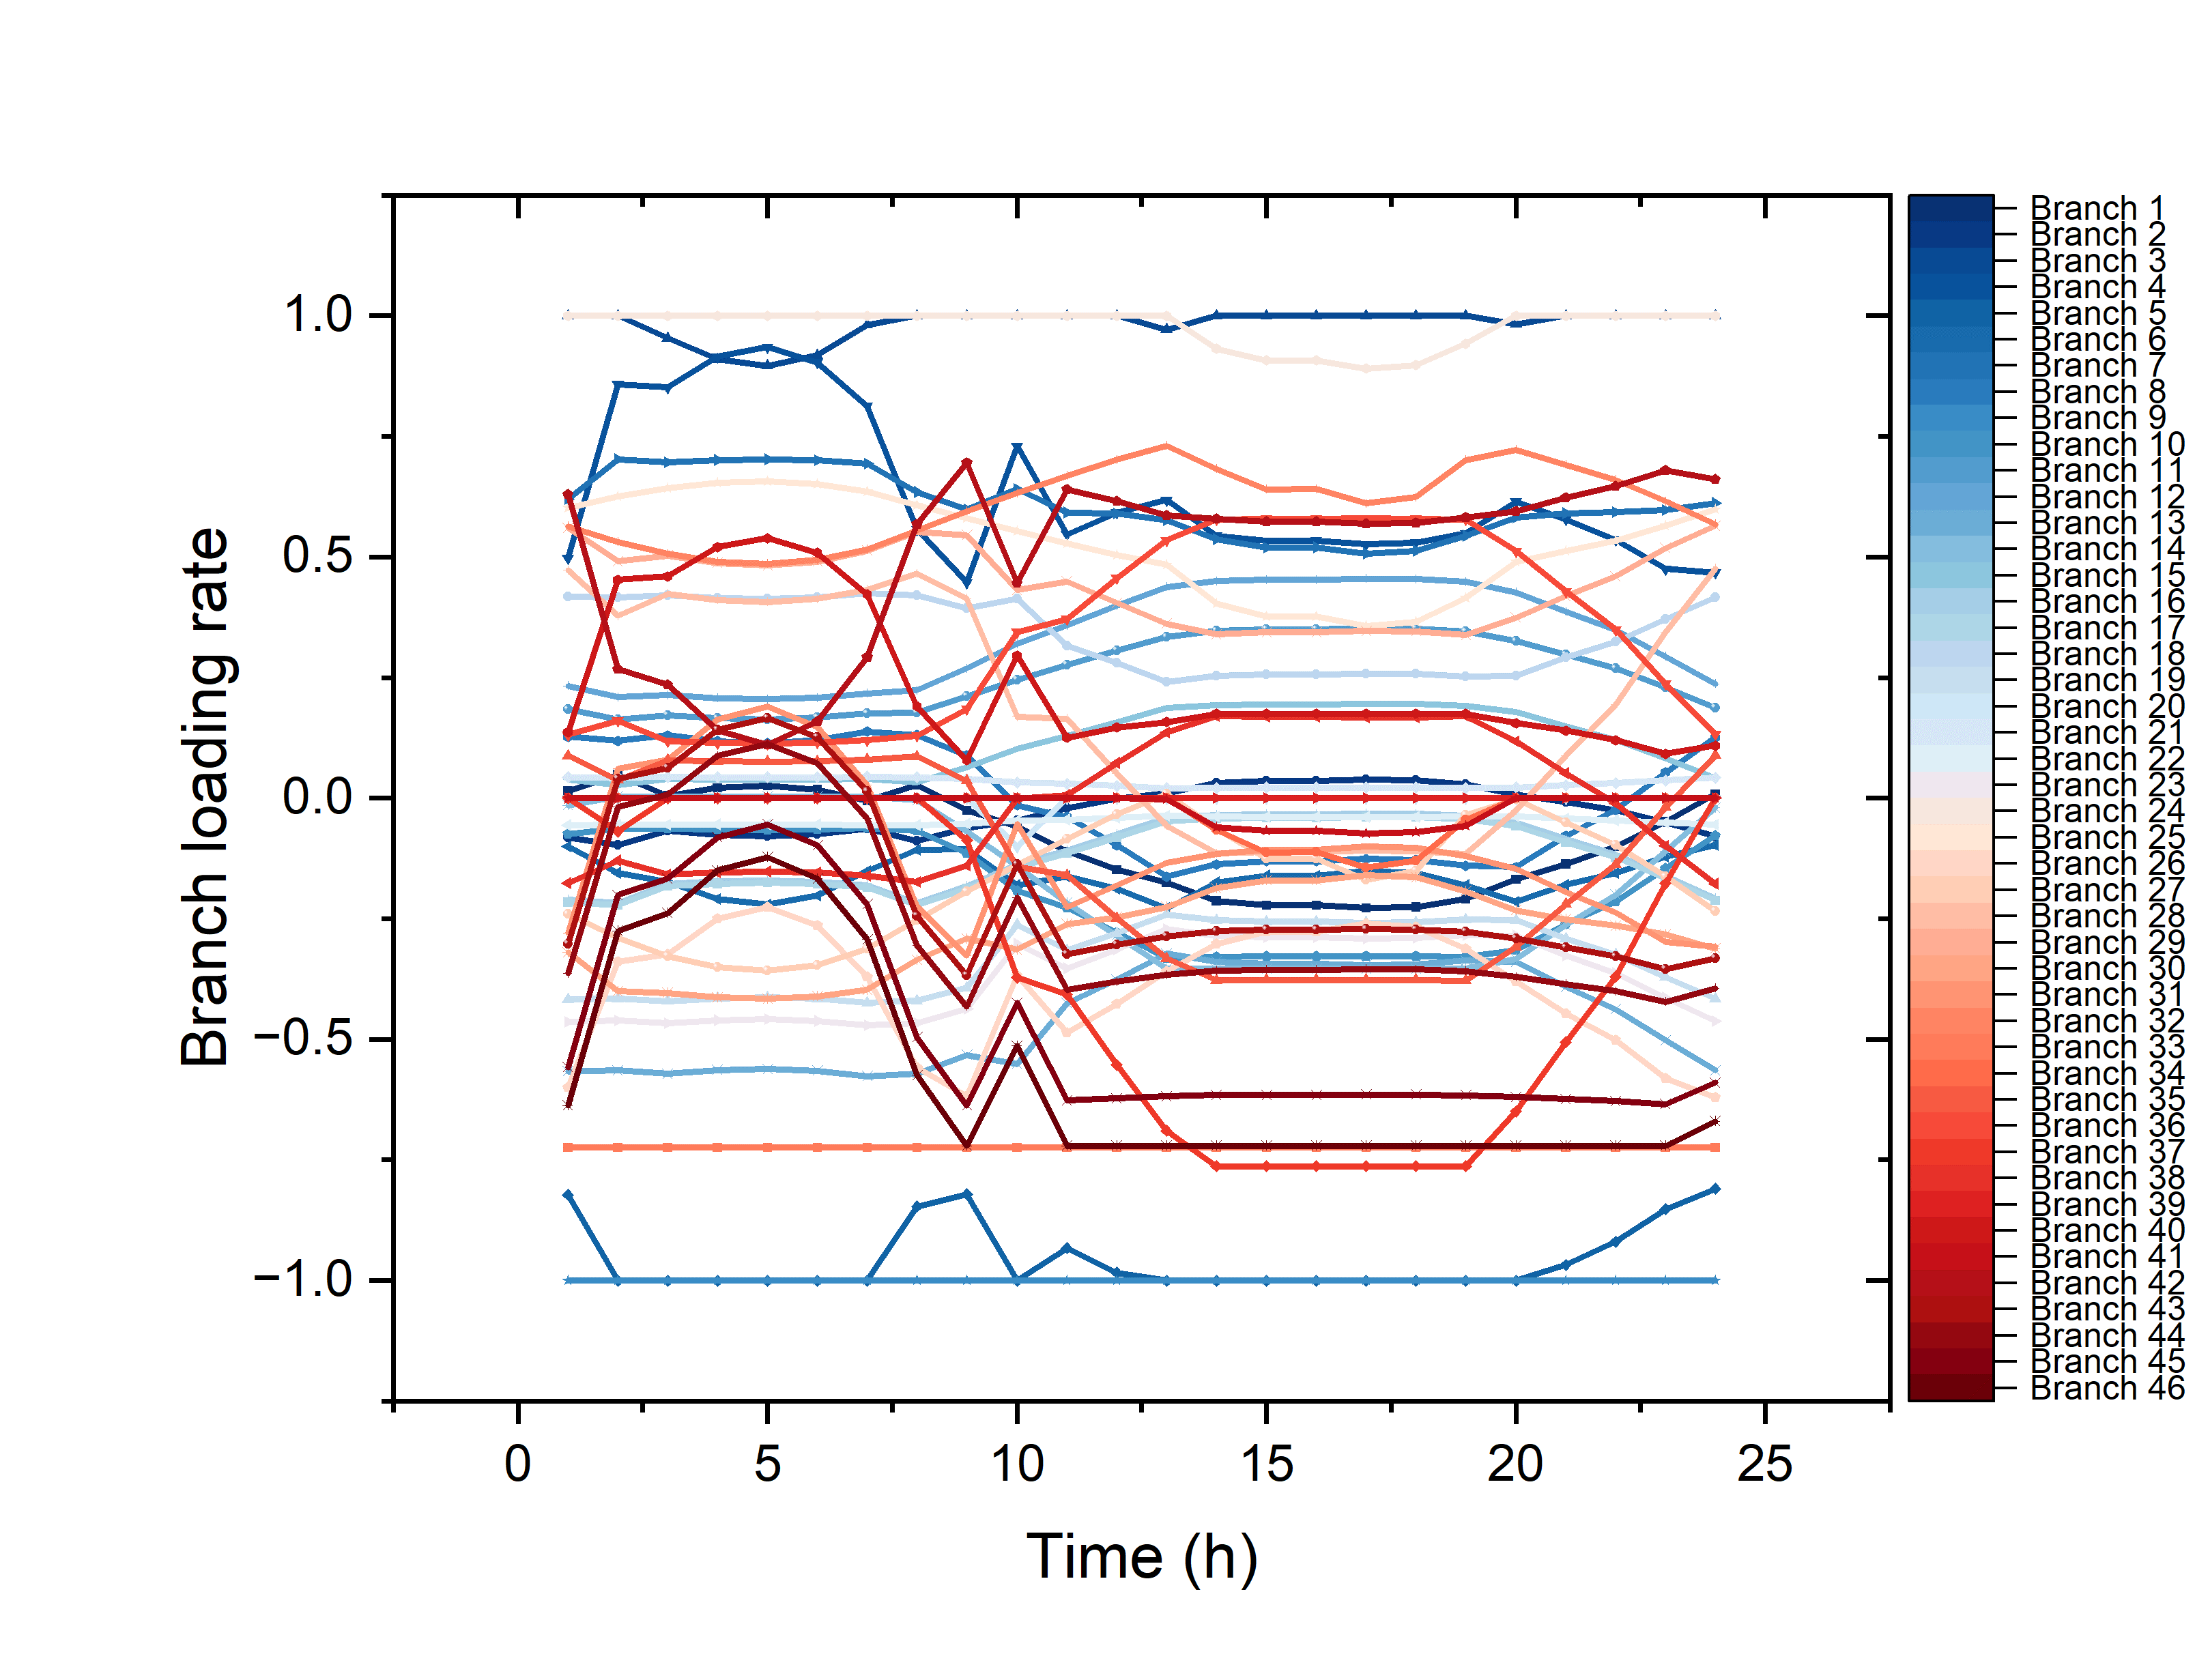
\includegraphics[width=0.5\textwidth]{t2-br-wr0.5}
	\caption{The branch loading rate for different time intervals (wind rate = 0.5)}
	\label{fig_2}
\end{figure}

Fig. 10  illustrates the variation in load rates across different time intervals for two transmission branches (Branch 4 and Branch 13) under varying wind penetration rates (0.1, 0.25, and 0.5). The load rate represents the proportion of the branch's capacity being utilized, with values closer to 1 indicating higher utilization and values closer to -1 indicating lower utilization.

In Branch 4, it can be observed that as the wind penetration rate increases from 0.1 to 0.5, the load rate exhibits a decreasing trend, suggesting a reduction in the branch's capacity utilization. Conversely, for Branch 13, the load rate demonstrates a mixed response to changes in wind penetration rates. Specifically, at lower wind penetration rates (0.1 and 0.25), the load rate tends to fluctuate, while at a higher penetration rate (0.5), the load rate stabilizes, albeit at a lower level compared to the other rates.

These observations highlight the complex interplay between wind power integration and transmission branch utilization, emphasizing the need for careful monitoring and management of grid operations to ensure optimal performance and reliability.

\begin{figure}
	\centering
	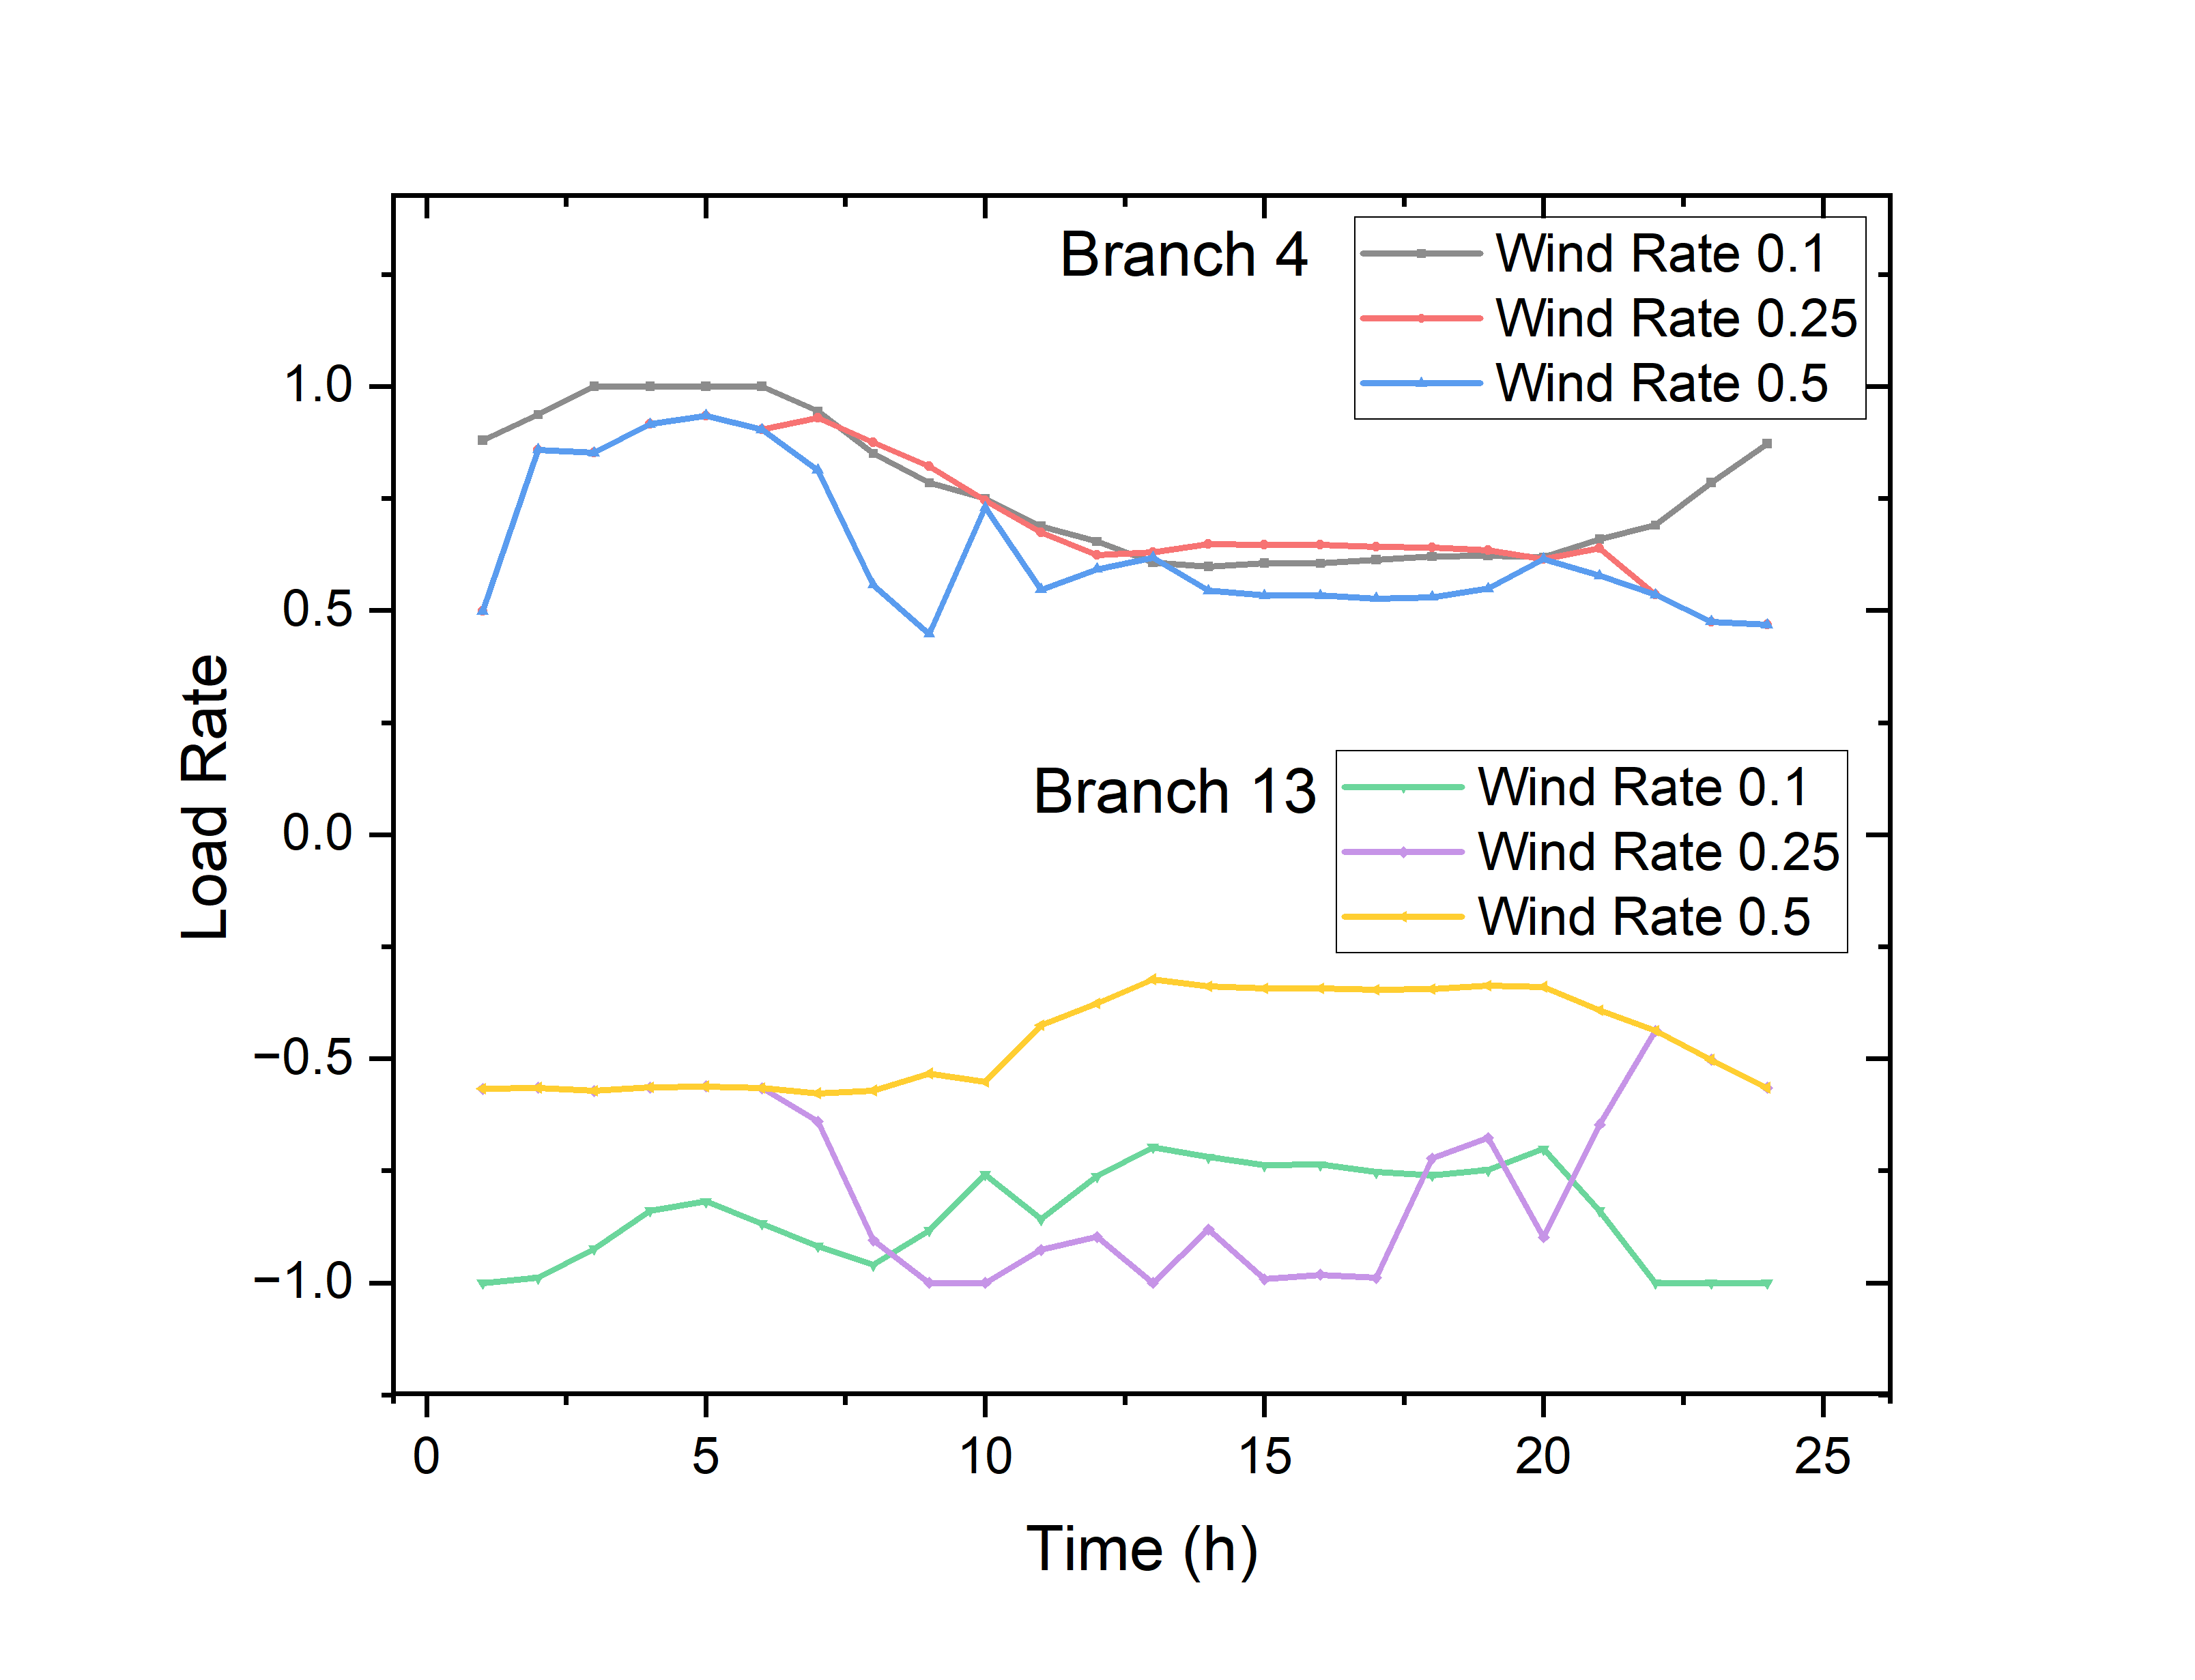
\includegraphics[width=0.5\textwidth]{t2-difwr}
	\caption{The branch loading rate for different time intervals (Branch 4\&13)}
	\label{fig_2}
\end{figure}


\subsection{Summarize and find out the potential impact}
Now we summarize and find out some potential impact of increasing wind power penetration level on system operation.

$\bullet$ Cost Reduction Potential: Increasing the penetration level of wind power in a system holds the potential to significantly reduce the total operating costs. Wind power, being a renewable energy source with zero fuel costs, can displace conventional generation sources, thereby mitigating the reliance on costly fossil fuels. As a result, the overall operational expenses associated with fuel procurement and generation can be diminished. Additionally, the integration of wind power can contribute to the reduction of greenhouse gas emissions, leading to potential environmental and societal benefits.

$\bullet$ Generation Dispatch Flexibility: A higher penetration level of wind power introduces greater flexibility in generation dispatch strategies. Traditional generation units, such as thermal and hydroelectric plants, may experience decreased utilization rates as wind power increasingly contributes to meeting system demand. This phenomenon, known as "generation curtailment," occurs when the output from conventional generators is scaled back to accommodate the variability of wind generation. Consequently, some generation units may operate intermittently or at reduced capacities, adjusting their output in response to fluctuations in wind power availability. This adaptive generation dispatch approach optimizes system efficiency and resource utilization while ensuring grid stability and reliability.

$\bullet$ Impact on System Dynamics: The integration of wind power alters the dynamic behavior of the power system, influencing key performance metrics such as generation adequacy, voltage stability, and frequency regulation. With higher levels of wind penetration, system operators must carefully manage the variability and uncertainty associated with wind generation to maintain grid stability. Advanced forecasting techniques, real-time monitoring, and responsive control mechanisms are essential for effectively integrating wind power into the grid and mitigating potential operational challenges.

In summary, increasing the penetration level of wind power offers multifaceted benefits for system operation, including cost reduction, enhanced generation dispatch flexibility, and dynamic system optimization. However, careful planning, advanced technologies, and robust operational strategies are crucial to harnessing the full potential of wind energy while ensuring the reliability and resilience of the power system.

\section{Security-constrained unit commitment (SCUC)}
Security-constrained unit commitment (SCUC) problem is one of most important tools in modern power system control center and electricity market. Also, we consider an energy storage system in this model.
\subsection{Use YALMIP to establish the multi-period OPF model and optimize}
\subsubsection{Data processing}
Based on the IEEE 39-bus system, wind generator is installed on bus 14 and ESS is installed on bus 13 and initial stored energy $E_0=0.2E_{cap}$. Load data and wind perdition data is stored in the "Data for SCUC" sheet of the DATA.xlsx. Set the load ratio to 1. SOC is defined as follows:
\begin{equation}
	SOC=\frac{E_t}{E^{cap}}
\end{equation}

Based on these data, firstly define decision variables. Newly defined decision variables includes $u$, which represent the on-off status of generator, $y$, which represent the start of generator. $xc$ and $xc$ represent whether charge and discharge power of ESS, $uc$ and $us$ represent charging and discharging status of ESS, $E$ represent the stored energy of ESS.
\begin{lstlisting}
	x = sdpvar(Nunits,Horizon,'full');
	theta=sdpvar(Nbus,Horizon,'full');
	xw= sdpvar(1,Horizon,'full');
	% Unit binary variables
	u=binvar(Nunits,Horizon,'full');
	y=binvar(Nunits,Horizon,'full');
	% ESS binary variables
	xc=sdpvar(1,Horizon,'full'); % charge power of ESS at time
	xs=sdpvar(1,Horizon,'full'); % discharge power of ESS at time
	uc= binvar(1,Horizon,'full'); % the charging status of ESS
	us= binvar(1,Horizon,'full'); %  the discharging status of ESS
	E= sdpvar(1,Horizon,'full'); % the stored energy of ESS at time 
\end{lstlisting}

\subsubsection{Objective}
Based on the instruction file, the objective function should be modified as follows:
\begin{equation}
	f_{1}=\sum_{t=1}^{T}\sum_{i=1}^{NG}\left(c_{i}^{o}x_{i,t}+c_{i}^{l}u_{i,t}\right)+\sum_{t=2}^{T}\sum_{i=1}^{NG}c_{i}^{s}y_{i,t}\
\end{equation}
\begin{equation}
	f_{2}=\lambda\sum_{t=1}^{T}\left(Pw_{t}-x_{t}^{w}\right)
\end{equation}
\begin{equation}
	f=f_1+f_2
\end{equation}

So the MATLAB code is changed as follows:
\begin{lstlisting}
	Objective = 0;
	% Obj  f1
	for k = 1:Horizon
	Objective = Objective + C*x(:,k) + Cl*u(:,k);
	end
	for k = 2:Horizon
	Objective = Objective + Cs*y(:,k);
	end
	
	% Obj f2
	Lambda=10;
	f2=sum(Pw-xw);
	f2=f2*Lambda;
	Objective=Objective+f2;
\end{lstlisting}

\subsubsection{Constraints}
Several constraints must be considered in our optimization model to ensure its accuracy and effectiveness. These constraints encompass nodal power balance, branch flow, generator capacity, minimum up/down time for generators, and energy storage limitations. While all constraints are crucial, for brevity, we'll focus on the generator minimum up/down time and energy storage constraints in this discussion. The code is as follows:
\begin{lstlisting}
	% Generator minimum up/down time constraints
	for k = 2: Horizon
		Constraints = [Constraints, y(:,k) >= (u(:,k)-  u(:,k-1)) ];
	end
	
	for i = 1: Nunits
		t0=UT(i);
		for k = 2 : Horizon-t0 +1
			Constraints = [Constraints, sum(u(i,  k : k+t0-1)) >= t0*y(i,k)];
		end
		t0=UD(i);
		for k = 2 : Horizon-t0 +1
		Constraints = [Constraints, sum(u(i,  k : k+t0-1)) >= t0* ( u(i,k-1)-u(i,k) ) ];
		end
	end
	
\end{lstlisting}

The constraints related to ESS is as follows:
\begin{lstlisting}
	% ESS constraints
	eps=0.1;
	etac=0.9;
	etas=0.9;
	Ecap=1;  % In this case, SOC = E;
	E0=0.2*Ecap;
	
	Psmax = 50;
	Pcmax=Psmax;
	
	for k=1:Horizon
	Constraints = [Constraints, uc(:, k)+us(:, k) <= 1];
	Constraints = [Constraints, 0<= xc <= Pcmax * uc(:,k) ];
	Constraints = [Constraints, 0<= xs <= Psmax * us(:,k) ];
	Constraints = [Constraints, eps*Ecap<= E(:,k) <= Psmax*Ecap  ];  
	end
	
	
	for k=2:Horizon
	Constraints = [Constraints, E(:,k)==E(:,k-1) + etac*xc(:,k)-etas*xs(:,k) ];
	end
	Constraints = [Constraints, E(:,1)==E0+ etac*xc(:,1)-etas*xs(:,1) ];
\end{lstlisting}




\subsubsection{Optimization}
Lastly,  optimize and analyze the model. The optimization information is as follows:
\begin{figure}[htbp]
	\centering
	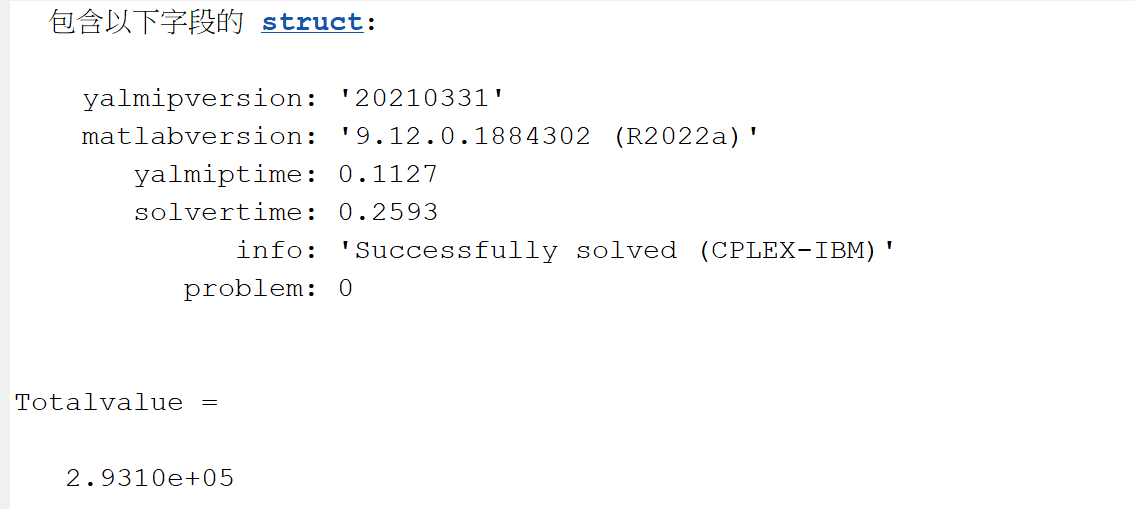
\includegraphics[width=0.5\textwidth]{t3-opt}
	\caption{The optimization information for SCUC problem (wind rate = 0.1)}
	\label{fig_2}
\end{figure}

The generator output and wind output variations across different time intervals are illustrated in Figure 12. It is noteworthy that the load power, representing the aggregate power demand, is determined by the combined power output from conventional generation sources and wind generation. Notably, the wind power component assumes a larger proportion of the load during non-peak time intervals compared to peak time intervals.

\begin{figure}[htbp]
	\centering
	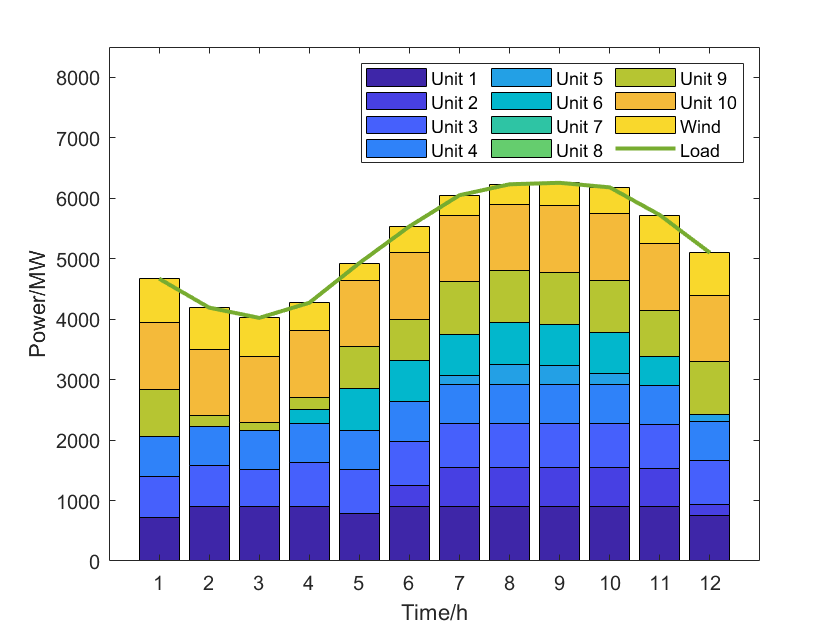
\includegraphics[width=0.5\textwidth]{t3-wr0.1}
	\caption{The generator output for different time intervals (wind rate = 0.1)}
	\label{fig_2}
\end{figure}


The branch loading rate and State of Charge (SOC) are depicted in Fig. 13 and Fig. The change trends of branch loading rate may align with, oppose, or be unrelated to variations in load. Additionally, the fluctuations in SOC exhibit an inverse relationship with the load curve, indicating that the Energy Storage System (ESS) undergoes charging during periods of low load (valley time) and discharging during periods of high load (peak time).

\begin{figure}[htbp]
	\centering
	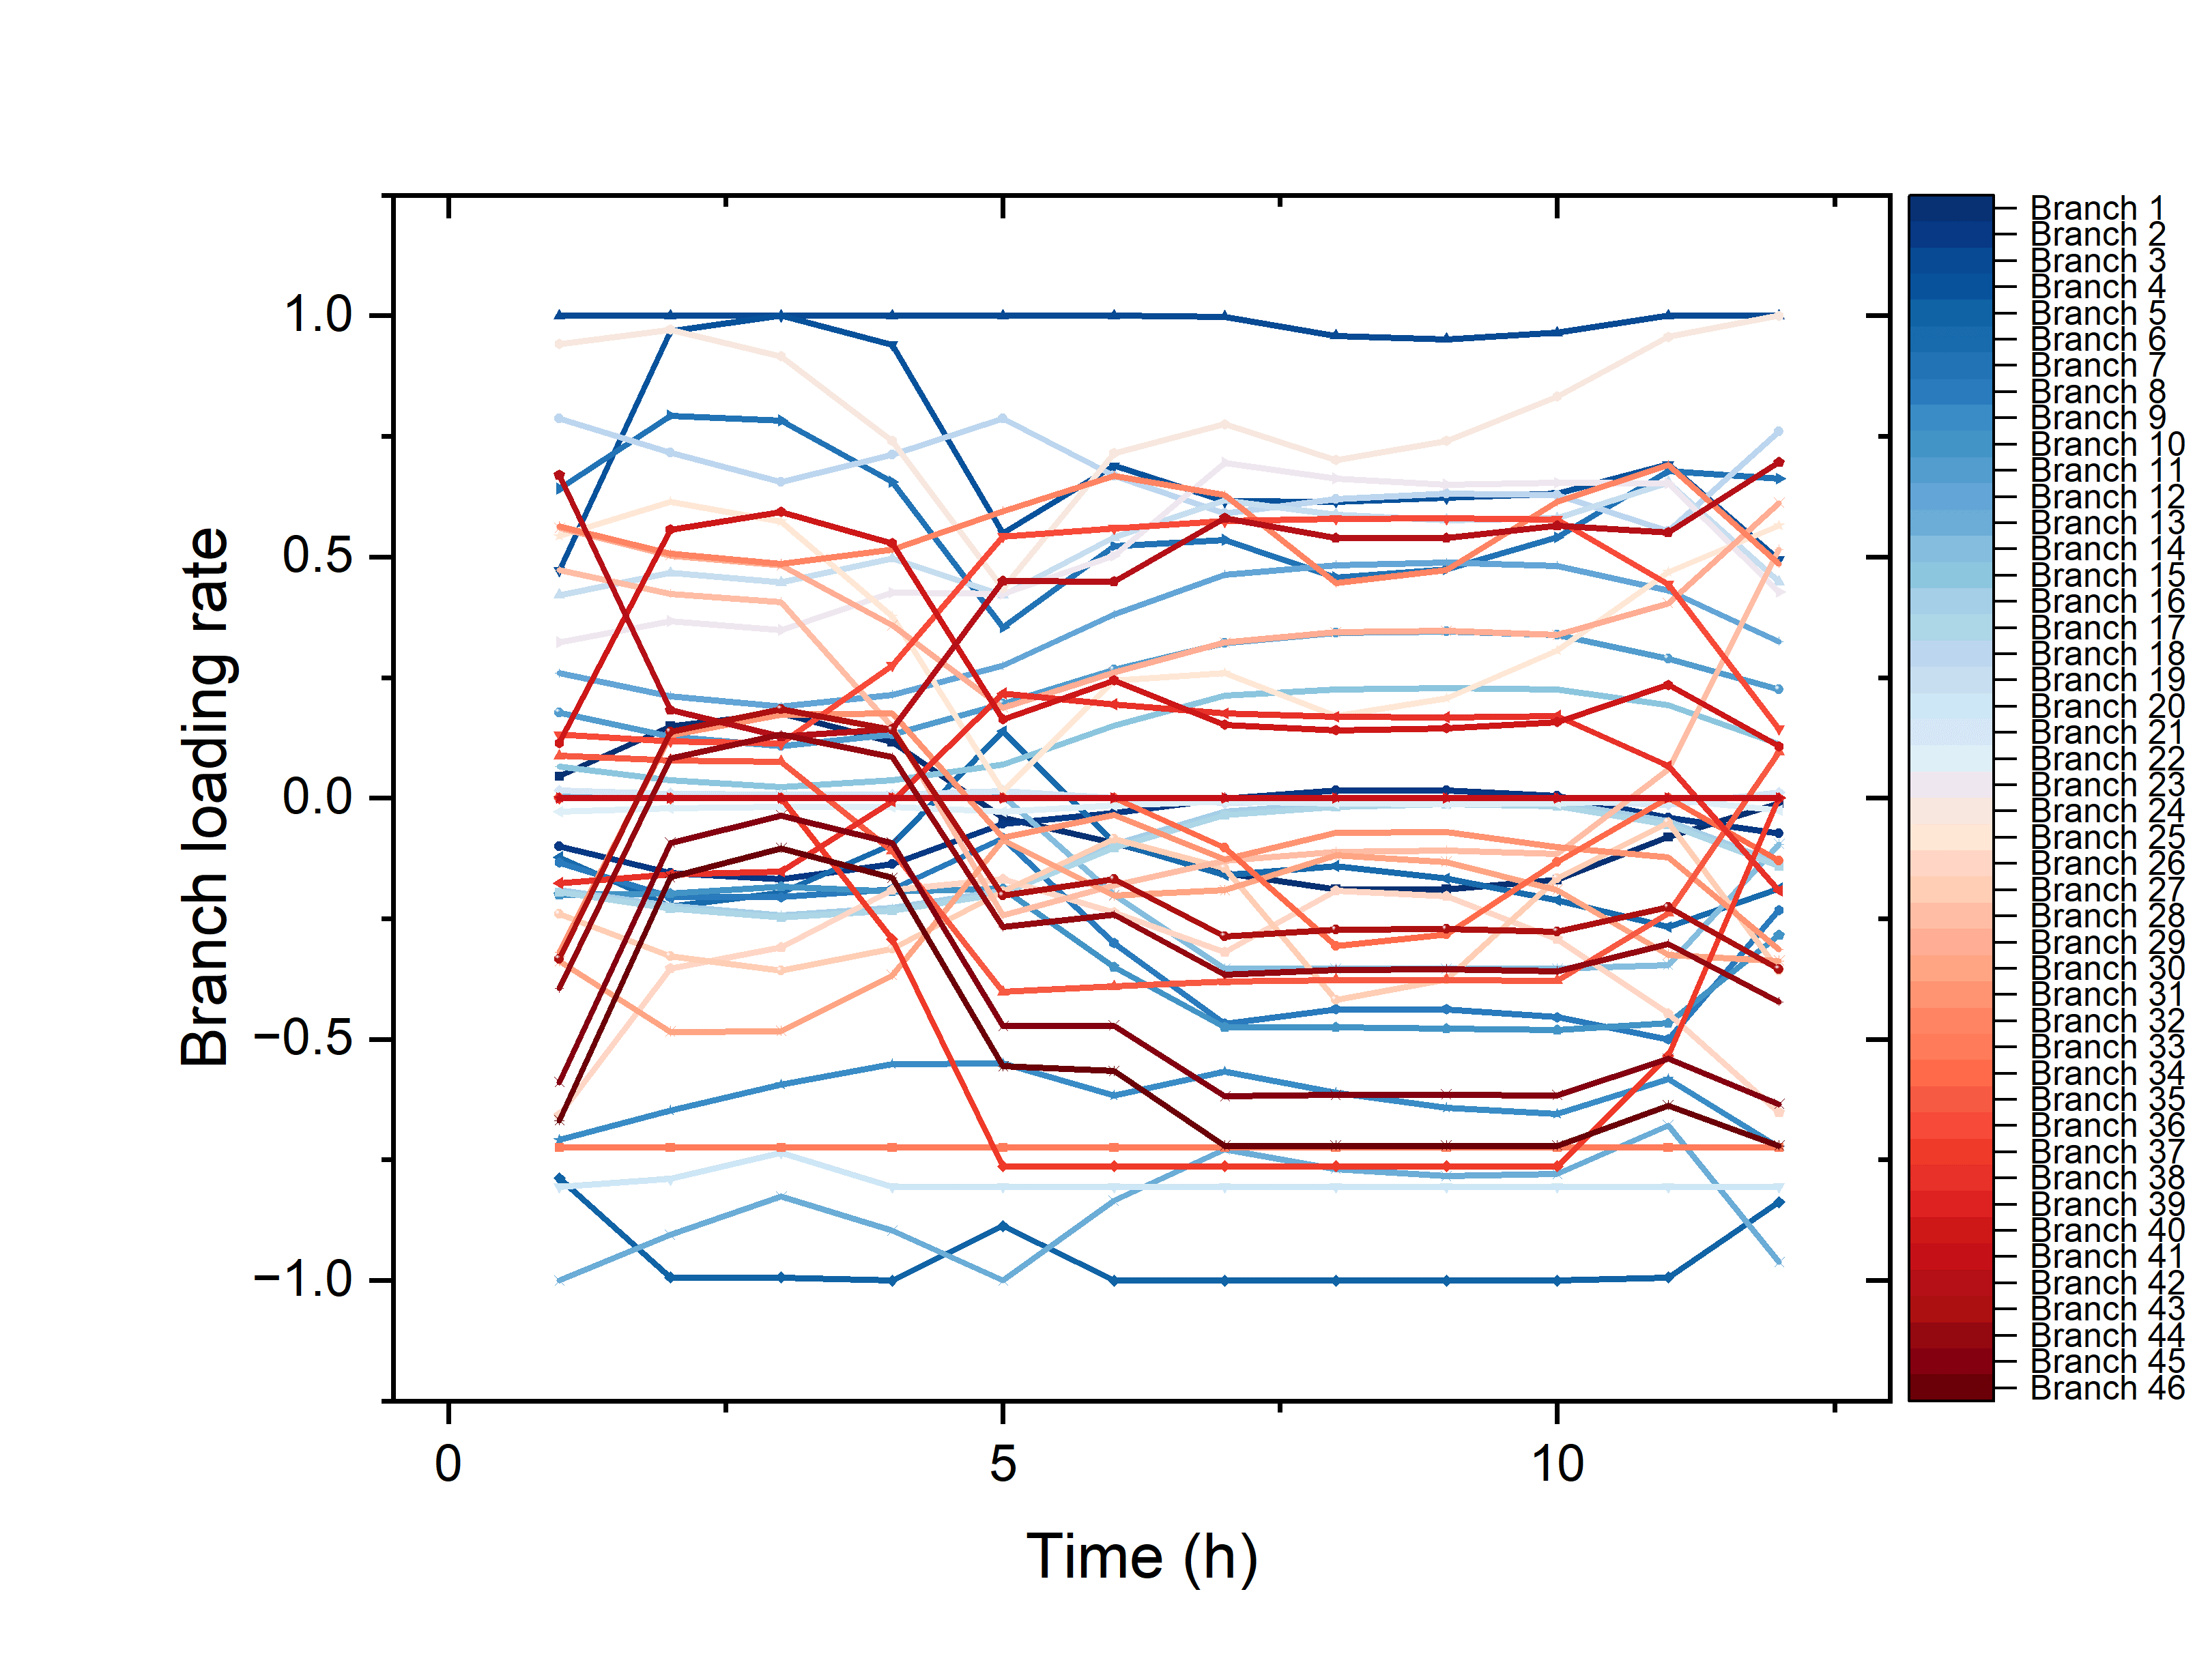
\includegraphics[width=0.5\textwidth]{t3-br-wr0.1}
	\caption{The branch loading rate output for different time intervals (wind rate = 0.1)}
	\label{fig_2}
\end{figure}

\begin{figure}[htbp]
	\centering
	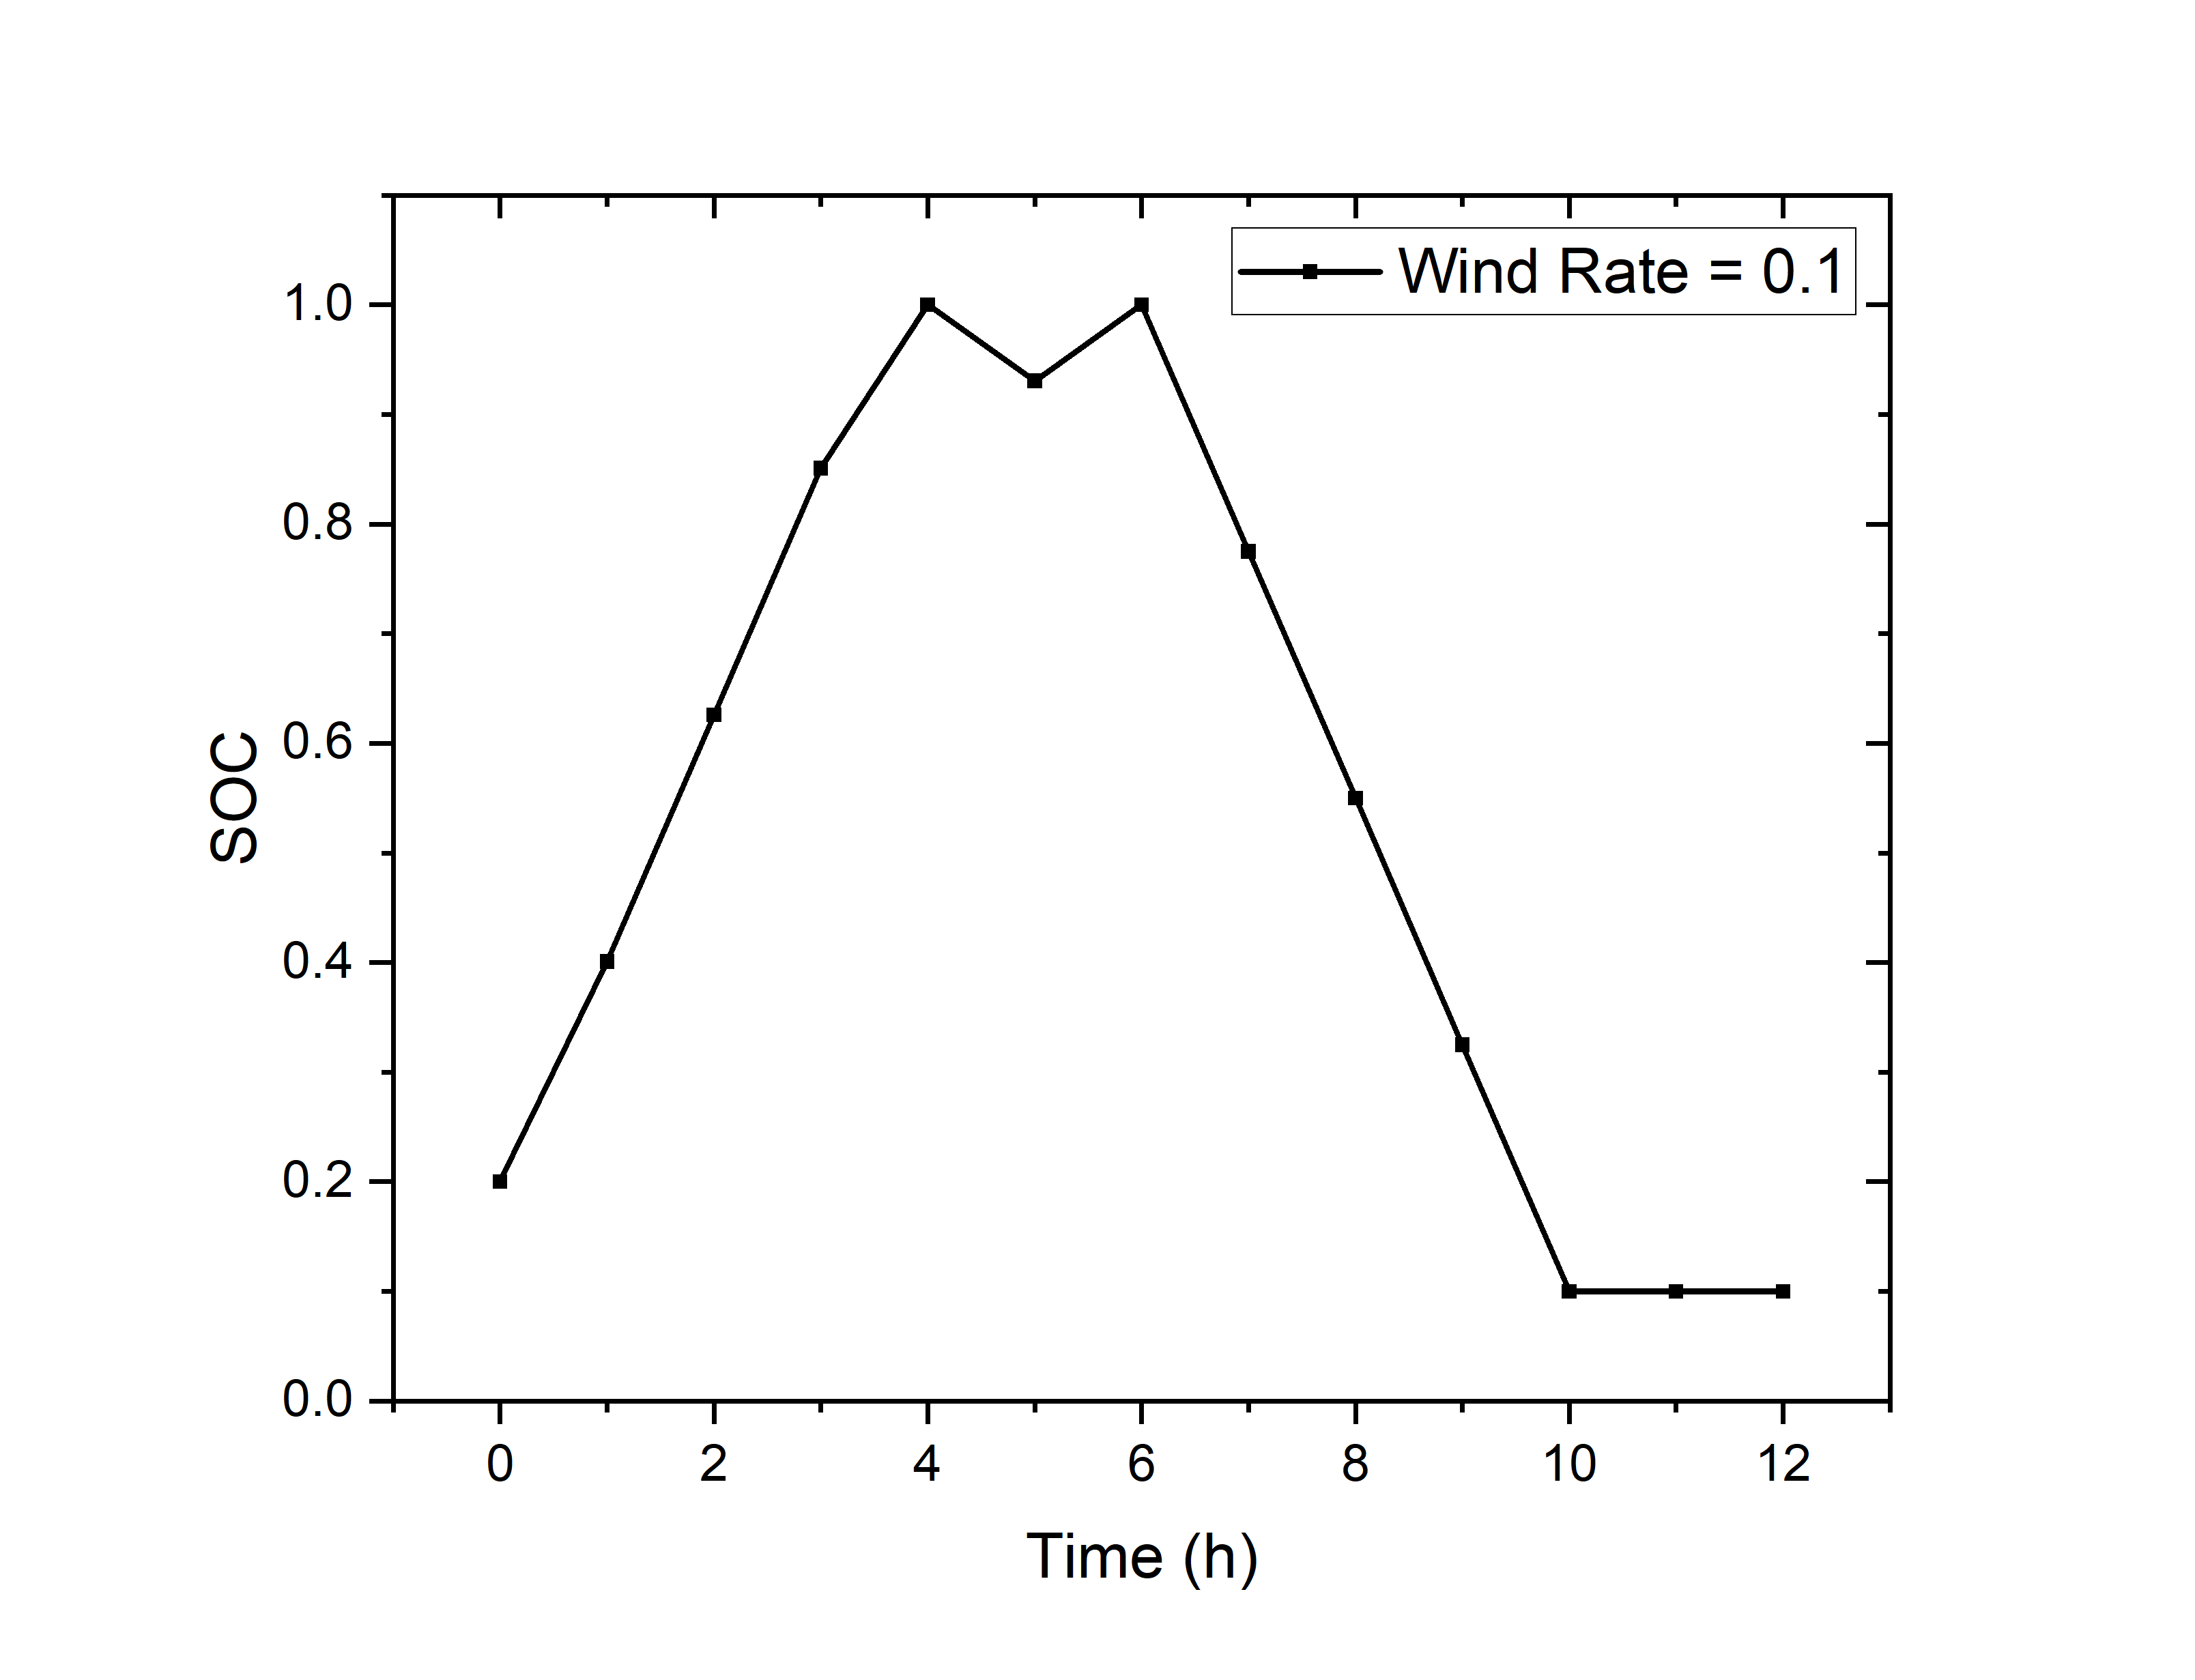
\includegraphics[width=0.5\textwidth]{t3-SOC-wr0.1}
	\caption{The SOC for different time intervals (wind rate = 0.1)}
	\label{fig_2}
\end{figure}

\subsection{Change the wind generator capacity}
In this section, we increase the capacity of the wind generator to 25\% and 50\% of the sum of generator capacity (excluding wind generator itself), use YALMIP to establish the model above and optimize, then observe the branch loading rate, the generator output, the wind output as well as SOC changes in different time intervals.

\begin{figure}[htbp]
	\centering
	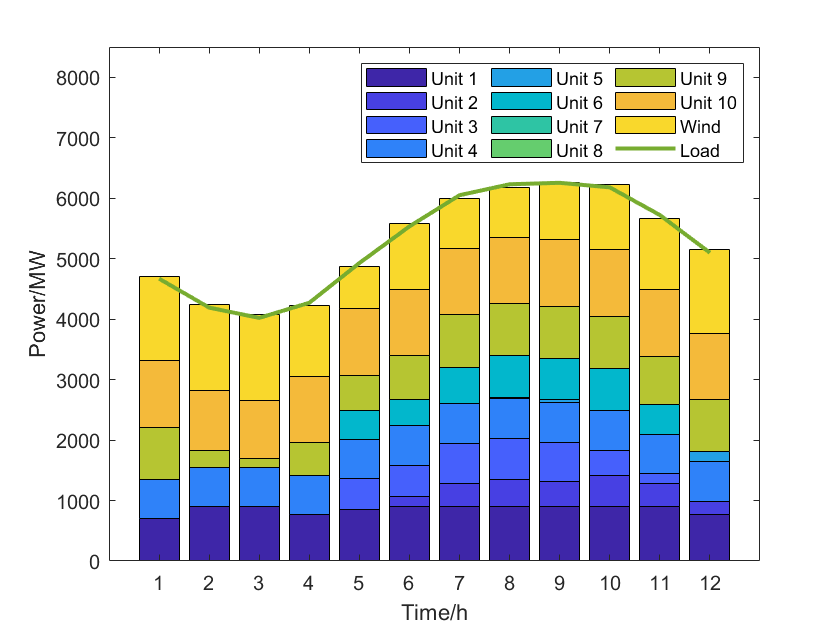
\includegraphics[width=0.5\textwidth]{t3-wr0.25}
	\caption{The generator output for different time intervals (wind rate = 0.25)}
	\label{fig_2}
\end{figure}

\begin{figure}[htbp]
	\centering
	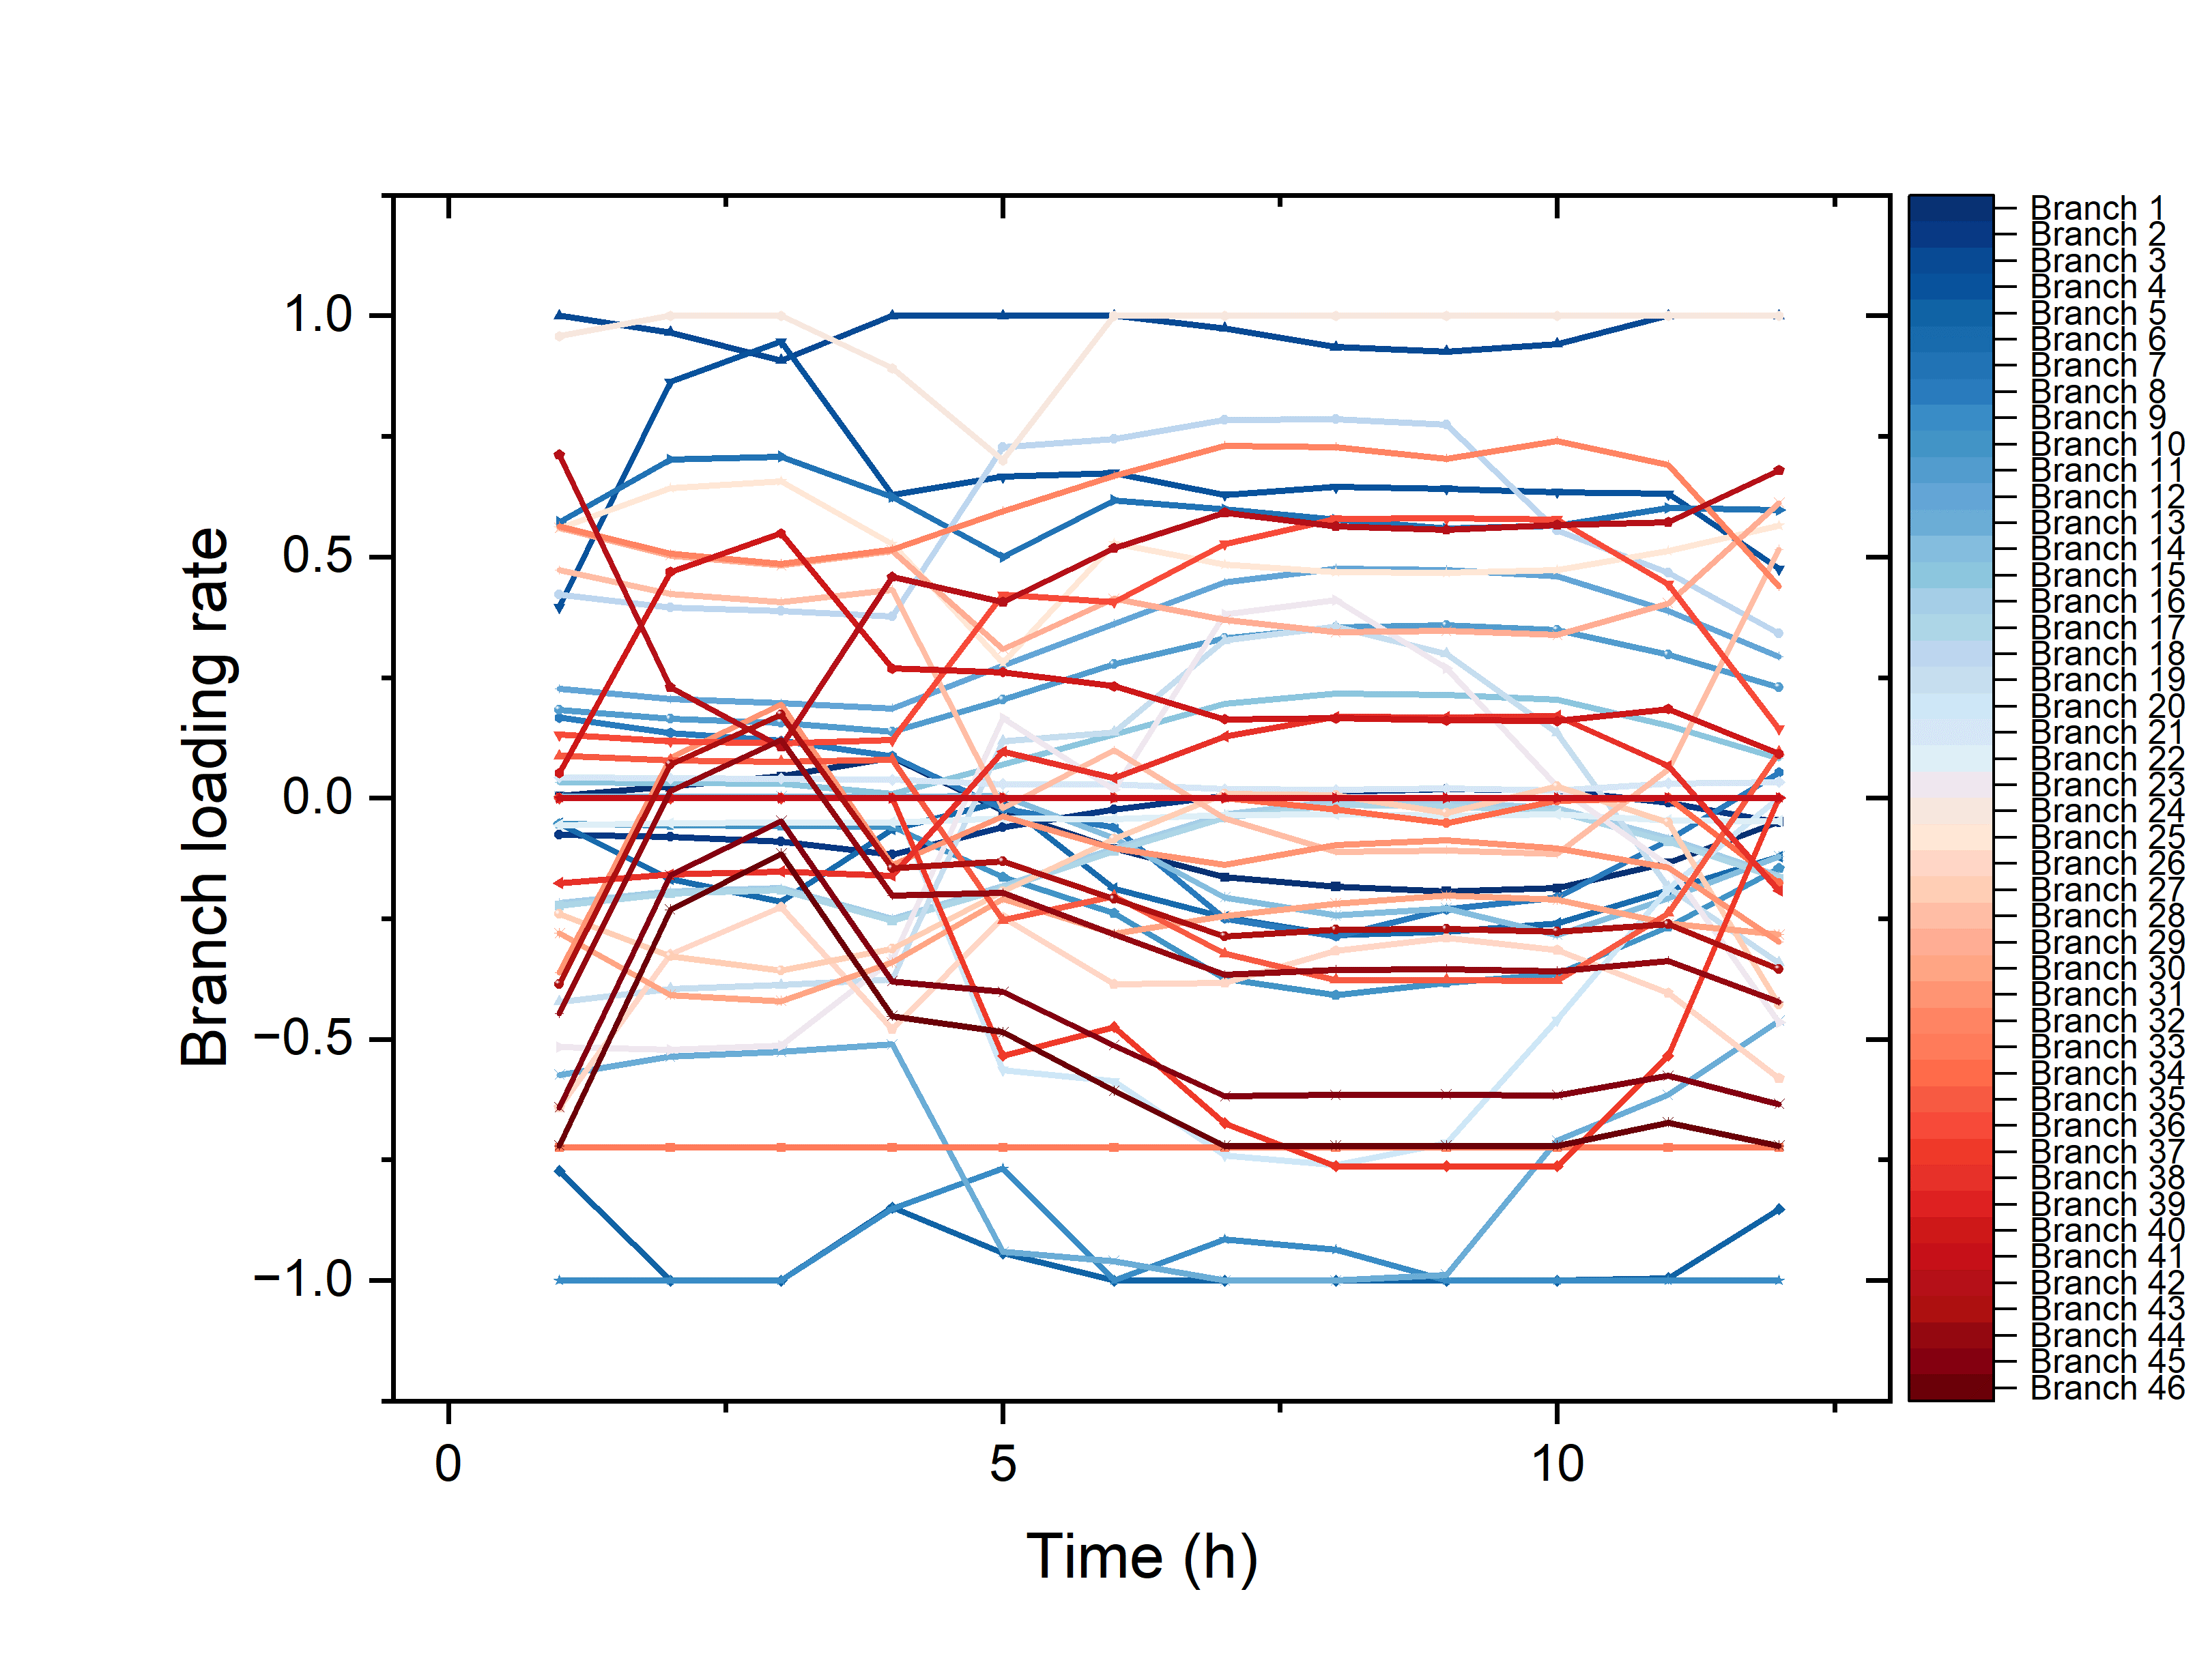
\includegraphics[width=0.5\textwidth]{t3-br-wr0.25}
	\caption{The branch loading rate output for different time intervals (wind rate = 0.25)}
	\label{fig_2}
\end{figure}

\begin{figure}[htbp]
	\centering
	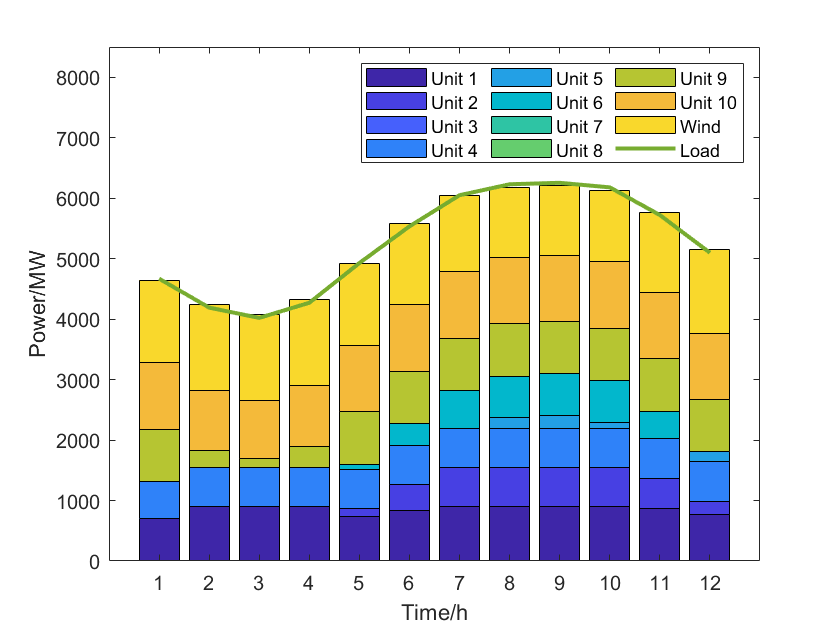
\includegraphics[width=0.5\textwidth]{t3-wr0.5}
	\caption{The generator output for different time intervals (wind rate = 0.5)}
	\label{fig_2}
\end{figure}

\begin{figure}[htbp]
	\centering
	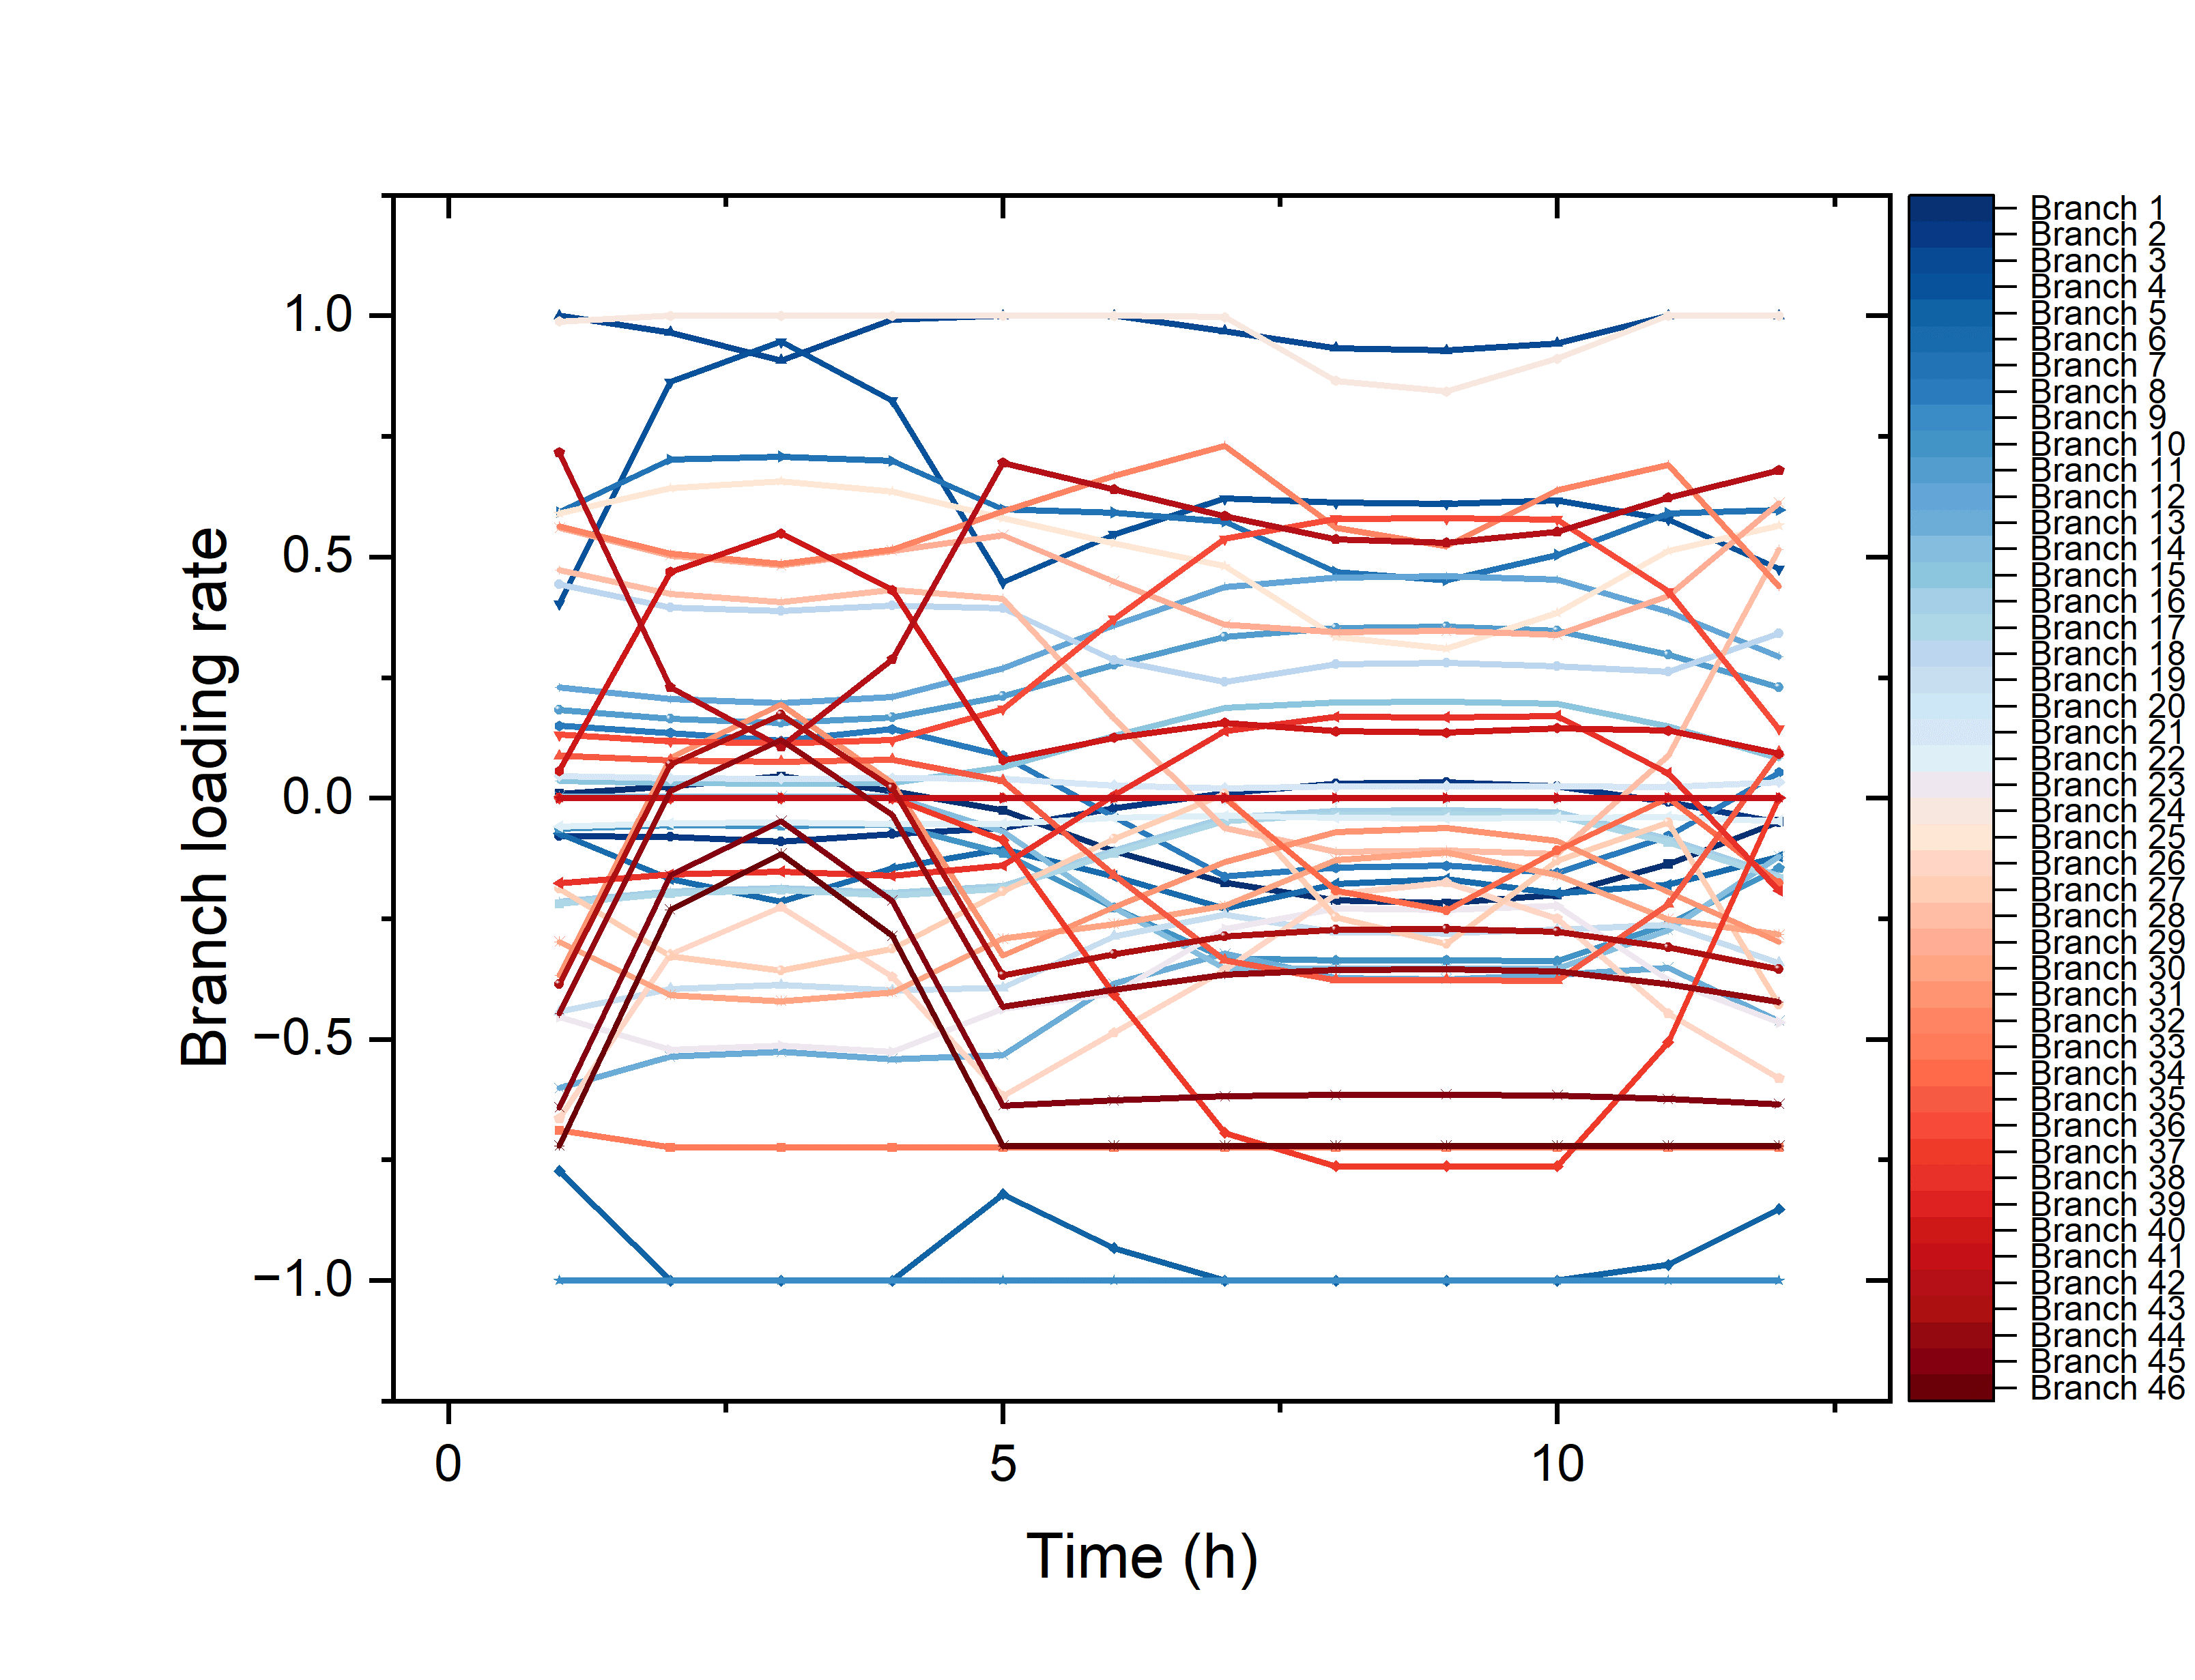
\includegraphics[width=0.5\textwidth]{t3-br-wr0.5}
	\caption{The branch loading rate output for different time intervals (wind rate = 0.5)}
	\label{fig_2}
\end{figure}

\begin{figure}[htbp]
	\centering
	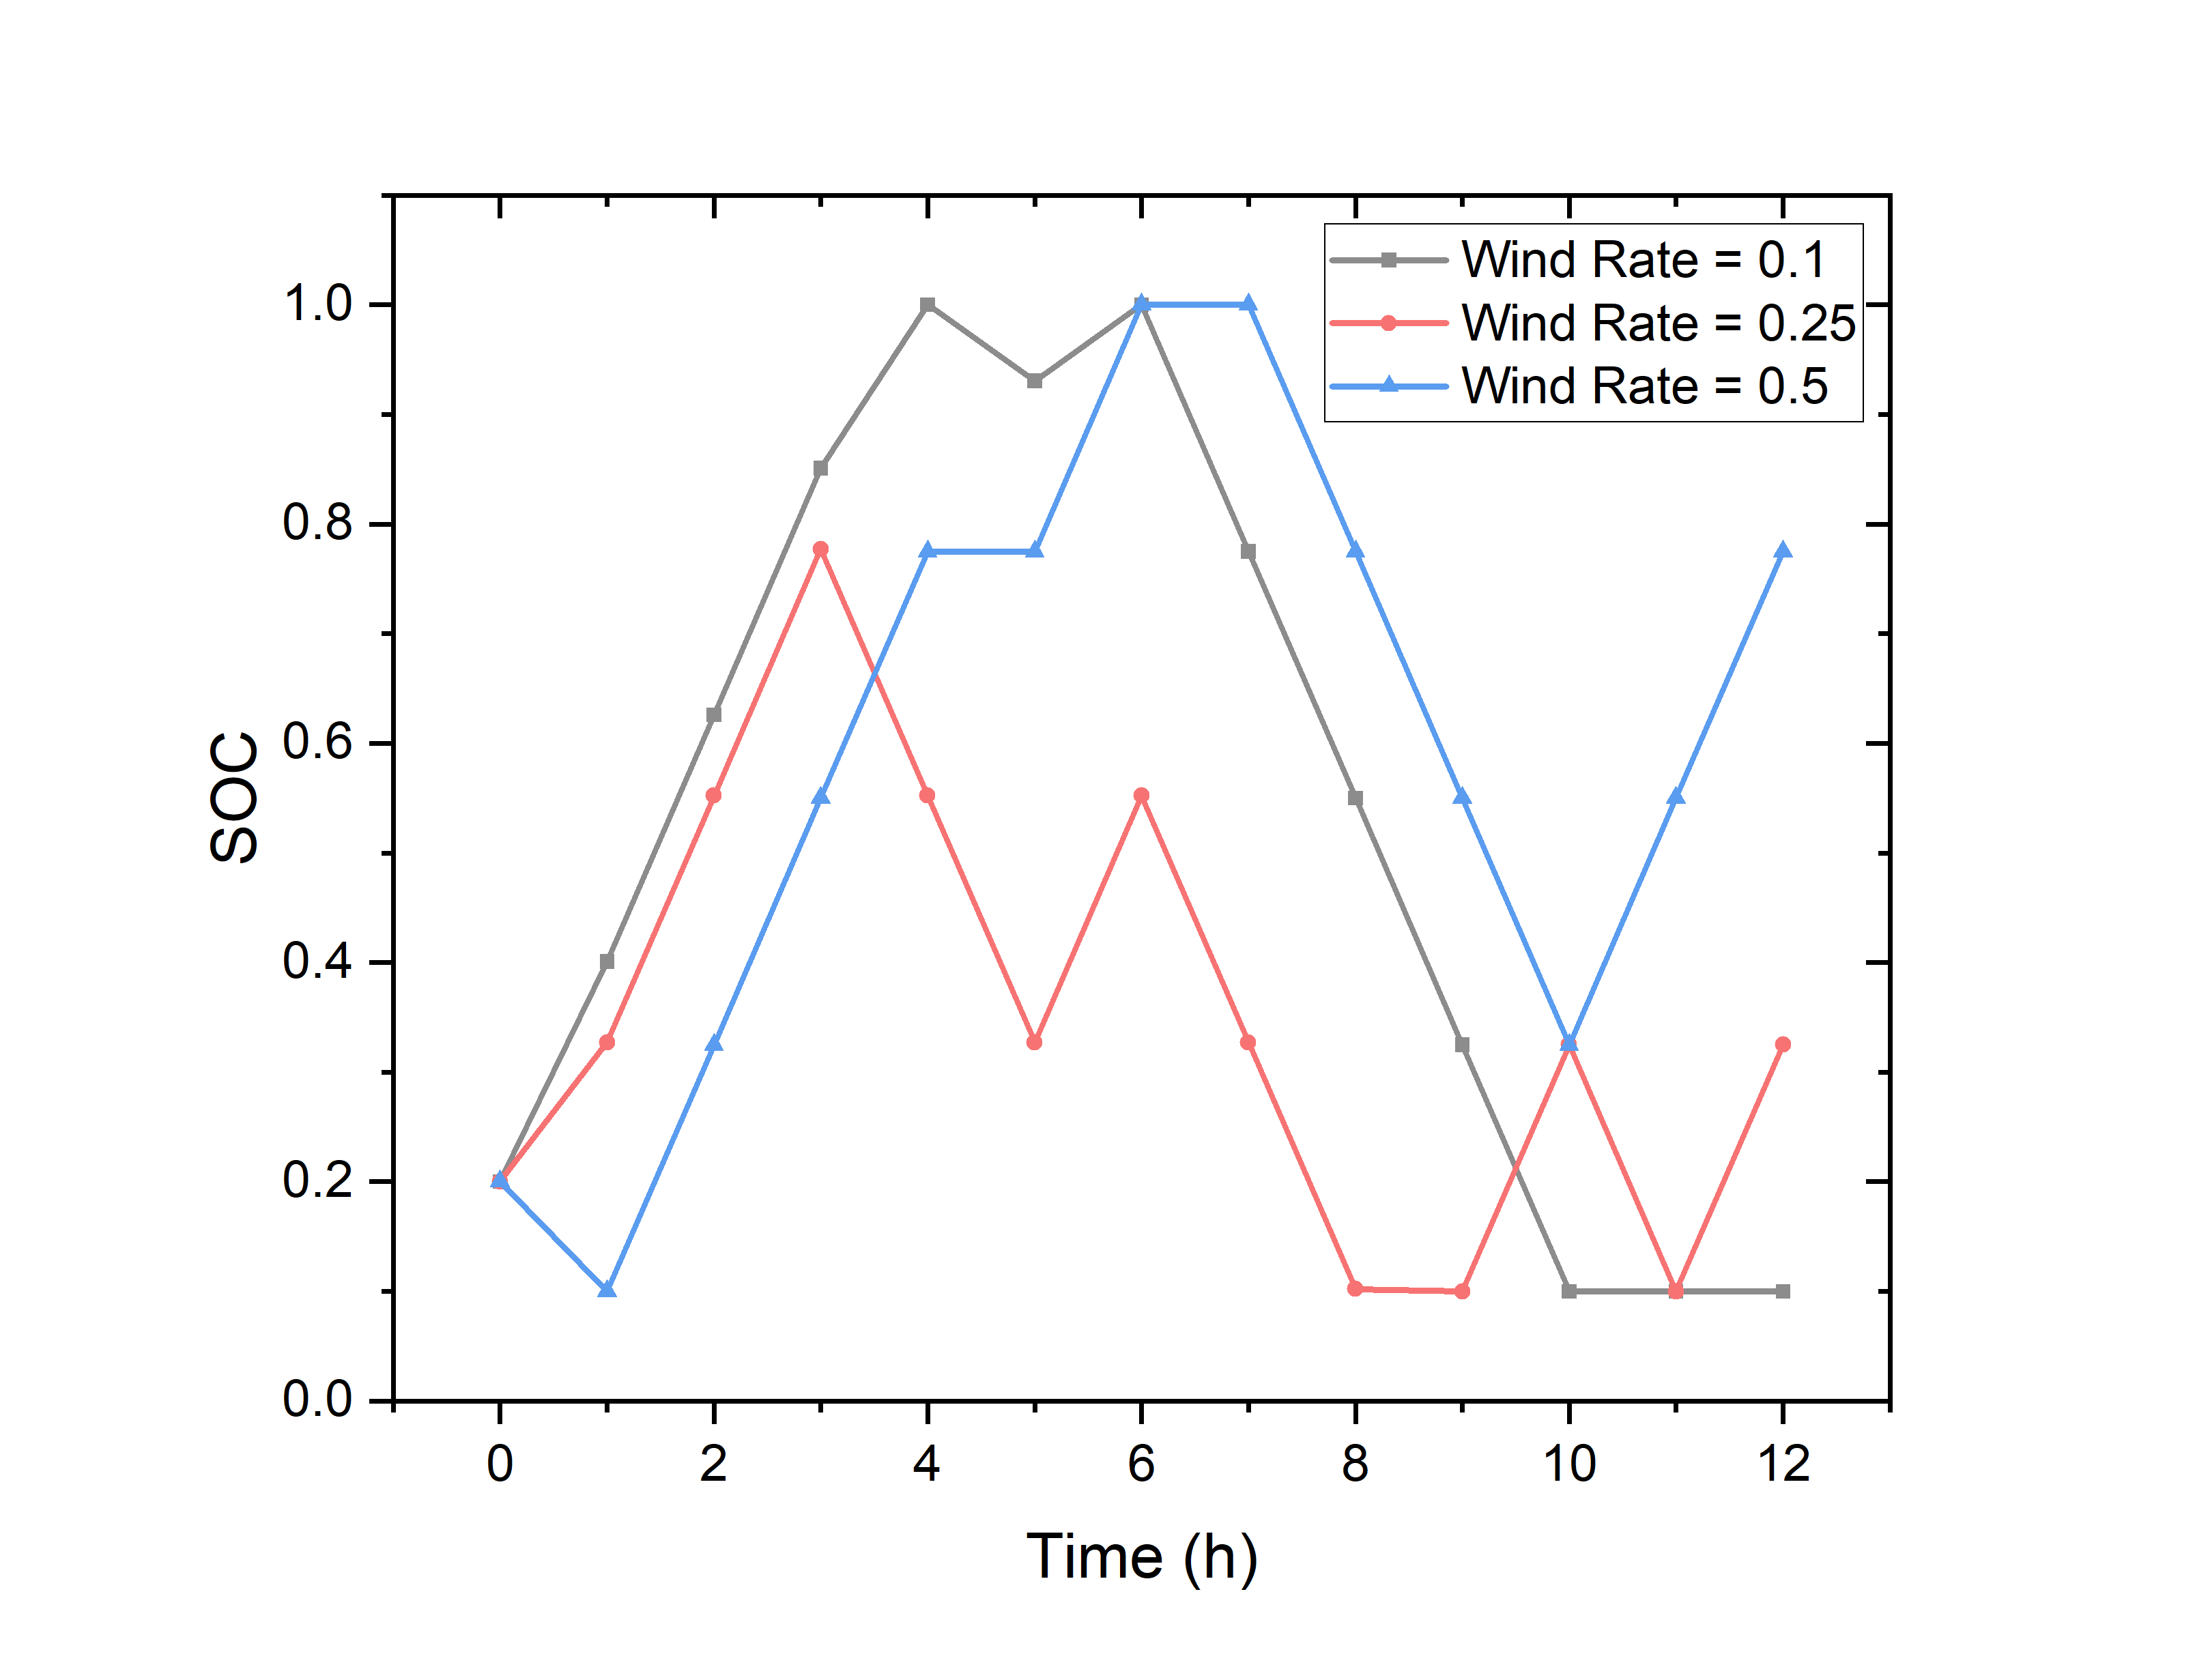
\includegraphics[width=0.5\textwidth]{t3-SOC}
	\caption{The SOC for different time intervals under different wind rate}
	\label{fig_2}
\end{figure}


Comparing with Fig. 13, where the wind power penetration level is only 10\%, it's evident that wind power constitutes an increasingly significant portion of the total power output in every time interval as the wind generator capacity grows, as illustrated in Fig. 15 and Fig. 17. Consequently, there is a decrease in the number of generators operating or operating at full capacity in each time interval, owing to the escalating power output from wind generators.

Additionally, as depicted in Fig. 16 and Fig. 18, the branch loading rate of branches tends to normalize with the expansion of wind generator capacity.

\subsection{Summarize and find out the potential impact of increasing wind power penetration level on system operation}

increasing wind power penetration level has several potential impacts on system operation:

$\bullet$ Shift in Power Generation: As wind power constitutes a larger proportion of total power output, there is a shift in power generation dynamics. Traditional generators may operate less frequently or at reduced capacities, leading to changes in overall system dispatch.

$\bullet$ Reduced Generator Operation: With higher wind power penetration, fewer traditional generators may be needed to meet demand, particularly during periods of high wind availability. This can lead to reduced fuel consumption and operating costs for thermal generators.

$\bullet$ Branch Loading and System Congestion: Changes in power flow patterns due to increased wind power can influence branch loading rates and system congestion. This may require adjustments to grid infrastructure or operational procedures to ensure safe and reliable operation.

$\bullet$ Charging and Discharging of Energy Storage: With wind power fluctuations, energy storage systems may experience varying charging and discharging cycles. Optimal utilization of energy storage resources becomes crucial to smooth out variability and enhance grid stability.

\subsection{Identify the role of ESS by comparing the UC solution with and without the ESS installation}
In MATLAB, change the following code to remove ESS.
\begin{lstlisting}
	% Ecap=200;  
	Ecap=0; 
\end{lstlisting}

The optimization problem information is shown in Fig. 20.
\begin{figure}[htbp]
	\centering
	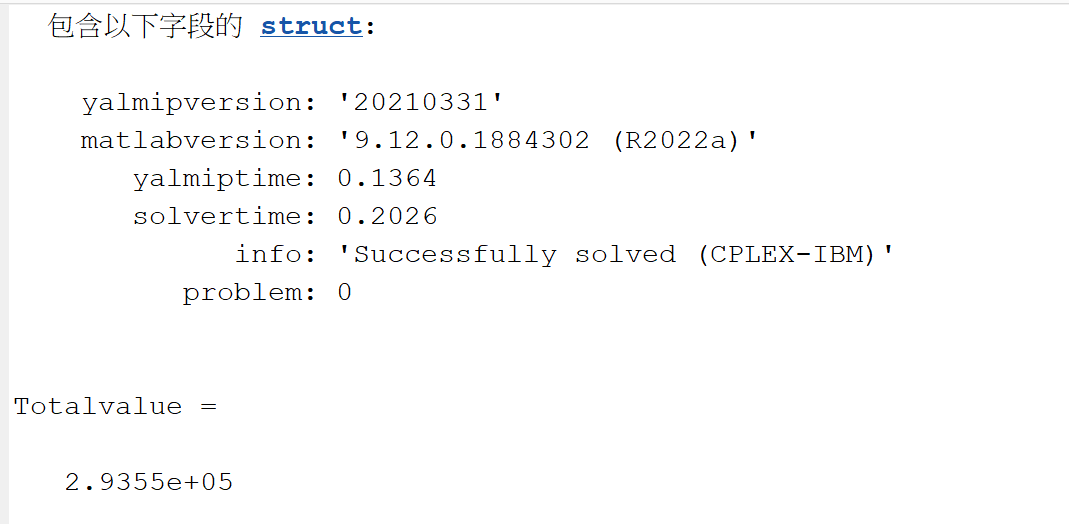
\includegraphics[width=0.5\textwidth]{t3-opt-noESS}
	\caption{The optimization problem information without ESS (wind rate =0.1)}
	\label{fig_2}
\end{figure}

Compared with Fig. 11, after removing the ESS, the optimal value of this SCUC problem rises from 293096.35 to 293547.41. It canbe seen that the installation of ESS can help reduce the totalcost (assuming that ESS has no cost).

\section{Acknowledgments}
I would like to express my sincere gratitude to our teacher,Guangchao Geng and teaching assistant, Jiajie Ling, for their invaluable guidance, support, and expertise throughout the duration of teaching. Their insightful feedback and encouragement have been instrumental in the successful completion of this project.






















\end{document}

